\documentclass[acmtog]{acmart}

\usepackage{booktabs} % For formal tables
\usepackage{multirow}

\usepackage[ruled]{algorithm2e} % For algorithms
\renewcommand{\algorithmcfname}{ALGORITHM}
\SetAlFnt{\small}
\SetAlCapFnt{\small}
\SetAlCapNameFnt{\small}
\SetAlCapHSkip{0pt}
\IncMargin{-\parindent}

% Metadata Information
\acmJournal{TOG}
\acmVolume{36}
\acmNumber{6}
\acmArticle{186}
\acmYear{2017}
\acmMonth{11}

% Copyright
%\setcopyright{none}
\setcopyright{acmcopyright}
%\setcopyright{acmlicensed}
%\setcopyright{rightsretained}
%\setcopyright{usgov}
%\setcopyright{usgovmixed}
%\setcopyright{cagov}
%\setcopyright{cagovmixed}

% DOI
\acmDOI{10.1145/3130800.3130895}

% use the "authoryear" citation style.
\citestyle{acmauthoryear}
\setcitestyle{square}

\input{99-Pre.tex}

% Document starts
\begin{document}


% Title portion
\title{Simplicial Complex Augmentation Framework for Bijective Maps}

%\author{Online Submission ID: 0375}

\author{Zhongshi Jiang}
\orcid{UNKNOWN}
\affiliation{%
   \institution{New York University}
   \streetaddress{60 5th Ave}
   \city{New York} 
   \state{NY} 
   \postcode{10011-8868}
 }
 \email{jiangzs@nyu.edu}

 \author{Scott Schaefer}
 \orcid{UNKNOWN}
 \affiliation{%
     \institution{Texas A\&M University}
   \streetaddress{3112 Texas A\&M University}
     \city{College Station} 
   \state{TX}
\postcode{77843-3112}
 }
 \email{schaefer@cs.tamu.edu}


 \author{Daniele Panozzo}
 \orcid{UNKNOWN}
 \affiliation{%
   \institution{New York University}
   \streetaddress{60 5th Ave}
   \city{New York} 
   \state{NY} 
   \postcode{10011-8868}
 }
 \email{panozzo@nyu.edu}


% The default list of authors is too long for headers}
\renewcommand{\shortauthors}{Z. Jiang et. al.}
\newcommand{\revise}[1]{#1}
\renewcommand{\revision}[1]{#1}


% The code below should be generated by the tool at
% http://dl.acm.org/ccs.cfm
% Please copy and paste the code instead of the example below. 
\begin{CCSXML}
<ccs2012>
<concept>
<concept_id>10010147.10010371.10010396</concept_id>
<concept_desc>Computing methodologies~Shape modeling</concept_desc>
<concept_significance>500</concept_significance>
</concept>
</ccs2012>
\end{CCSXML}

\ccsdesc[500]{Computing methodologies~Shape modeling}
%
% 
% End generated code
%

\thanks{This work was supported in part by the NSF CAREER awards IIS-1652515 and IIS-1148976, and a gift from Adobe}
Various applications, from artistic creation, to scientific computing, require the processing and reasoning of 3D digital objects.
The computational modeling of 3D geometric shapes, materials, and textures, as well as the simulation of their deformation and interactions, is essential to bring the algorithmic power of computing to real-life manufacture, architecture, and medical device design.
Depending on the specific numerical properties, better algorithm designs might prefer 3D data with different representations, for example, in planes, surfaces, or inside volumes.
This thesis investigates the problem related to the representations of data on 3D shapes and across different domains,
so computations for different stages within a pipeline, may come together synergistically without manual tuning that disrupts an automated data flow.
I propose novel geometrical principles in various geometric modeling and processing stages.
I also showcase various geometric computing applications that easily integrate such principles to guarantee the geometry validity and algorithm effectiveness of surface parameterization, rendering, deformation/animation, and mechanical simulation.
In addition, we can finally explore creative solutions that reliably coarsen the surface. Such simplification accelerates everyday geometric modeling operations; the contribution also includes a scalable method to construct coarse and curved meshes for fast animation and scientific computing.
Furthermore, the thesis provides a declarative way to formulate mesh processing and adaptation algorithms to facilitate the practical development of robust and reliable mesh processing software.
Finally, the thesis includes extensive numerical validations involving tens of thousands of complex geometry shapes. %And to maintain replicability and foster further research in this direction, I also released the implementation and generated data to be open source and accessible.

\begin{teaserfigure}
    \center
   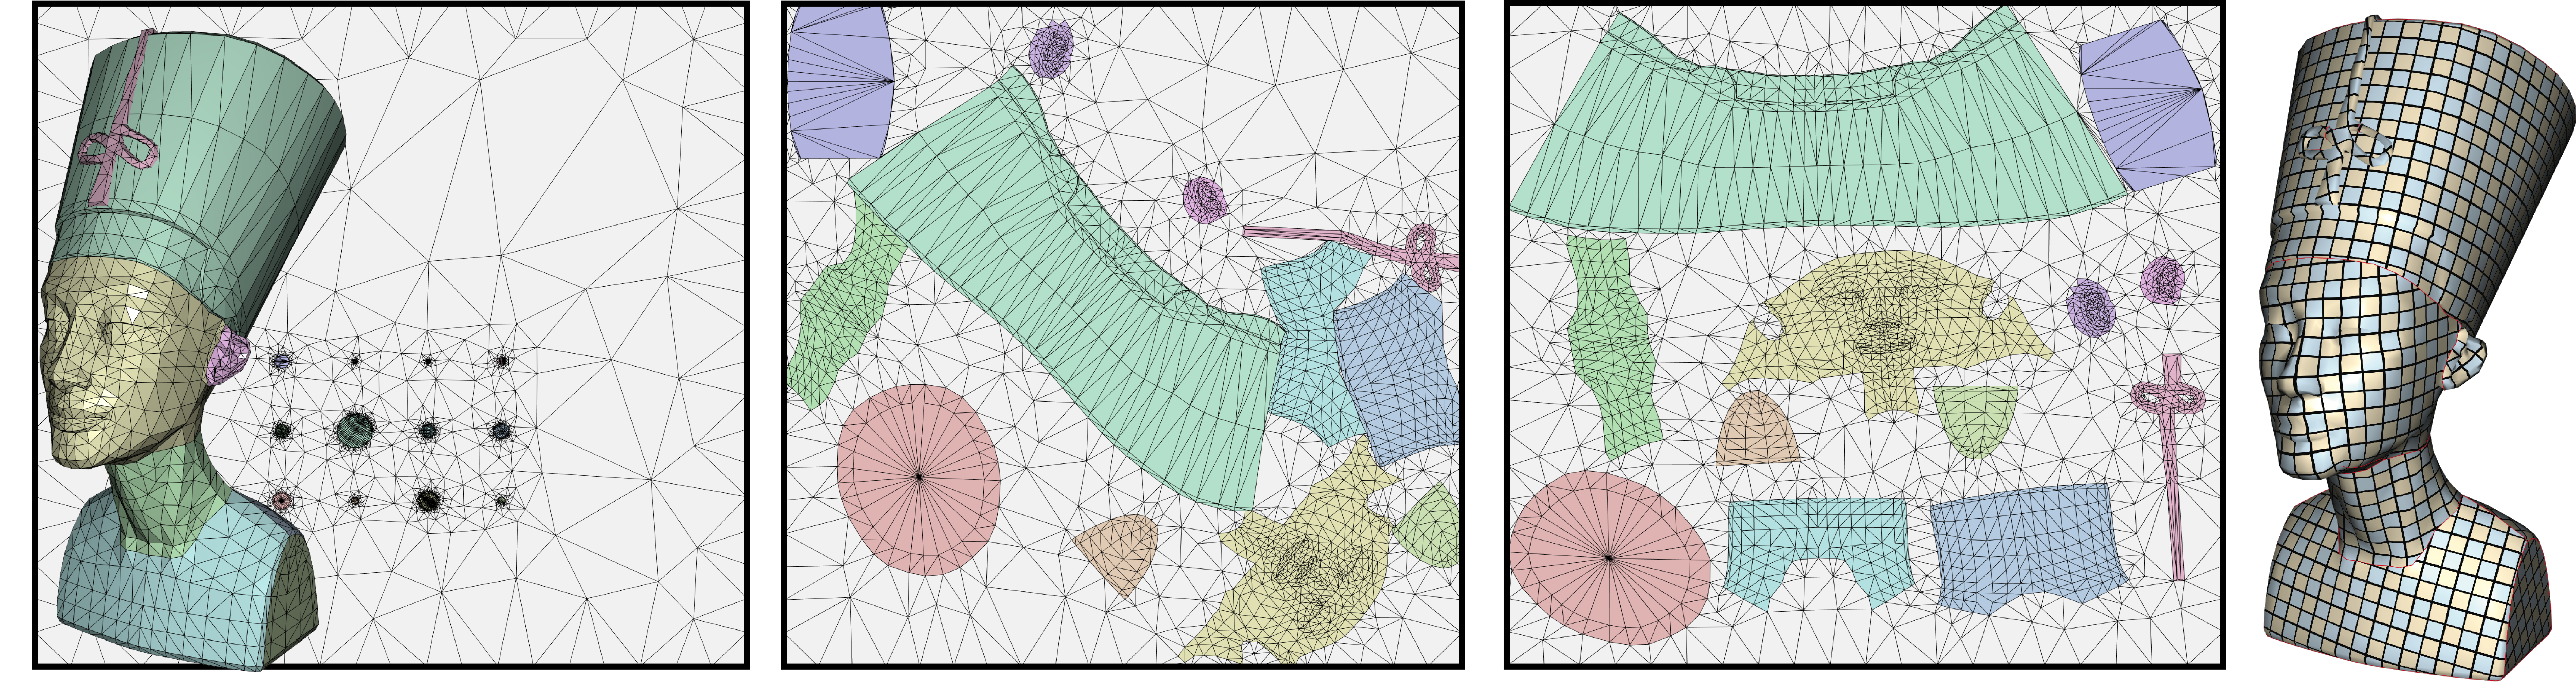
\includegraphics[width=\textwidth]{figs/teaser}
   \caption{The Nefertiti model with prescribed seams is UV mapped by our algorithm. Each chart is bijective mapped into a circle or ring with Tutte's embedding and achieves minimal distortion in less than a second. The layout is further improved interactively and the final parametrized model is shown on the right. Our approach guarantees a valid UV map with no inverted elements or overlapping triangles. See the attaching video for the optimization and manual interaction.
	}
   \label{scaf:fig:teaser}
\end{teaserfigure}



\maketitle

% background, modeling and simulation are connected through complex shape
% 

% We make our objects with manufacture pipeline, starting from a digital engineering design.
% advanced manufacturing and design techniques more and more complex shapes (engineering design).
Most of the everyday objects that we invent and interact in the physical world, ranging from electronic devices to transportation vehicles, are manufactured through a digital aided production pipeline.
First, given a desirable functionality, the designer compose a shape, then prototype and test the object under specified physical conditions. e.g. stress, or heat, or fluidic. 
Therefore, automatic computer algorithms for the design and fabrication would ensure the reliability and accessibility of medical devices. To do so requires a clear understanding of physical simulation and geometry design.

% On the other hand
On the other hand, composition of digital assets are through the similar pipeline, including human avatars, or objects that we are growing essential for the  virtual environment, thanks for 3D scanning techniques to obtain a digital shape, and then perform editing, fairing, modifications and other modeling operations. larger and larger quantites, and versatile of organic shapes beyond bunny. (scanning) and we want the dynamic deformation/collision response, in the information rich virtual environment, for interaction and physics based deformation.

% In both sides of these processes, there is the problem of robustness. And the need to connect modeling with simulation. and to process the information back and forth.
Researchers usually examine the computational design and physical simulation separately, leading to different computational tools for the discretized geometry. Different representations between design methods and various adaptations of simulations, even for the same shape, are not reliably correlated. In the general case, the material, attribute, or experiment setting cannot be robustly re-used on another representation without laborious manually fixing. Such a pipeline demands the engineer or designer to understand precisely the properties of the specific numerical methods of choice. It also prohibits an automatic and robust pipeline from optimizing the desired physical durability or permeability structure. 

\fbox{\parbox{0.9\textwidth}{\textcolor{gray}{
This dissertation is primarily concerned with the problem of how to effectively dealing with attributes, in various scenarios.
\begin{itemize}
  \item SCAF: representations to store attributes in plane, and applying such techniques to volume parameterization. This is crucial step for reliable attribute transfer between surfaces and volumes. color texture materials.
  \emph{Robust}, \emph{Deformation}, \emph{Geometry}.
\item SHELL: building on top, novel parameterization strategies between surfaces, for complex geometry, with nontrivial topology. \emph{Robust}. \emph{Simulations}, \emph{Geometry}. 
\item CURVE: application of shell, transfer serving robust simulation. \emph{Robust}. \emph{Simulations}, \emph{Geometry}. 
\item WMTK: speed up, robustness, aforementioned conditions, easily integrate constraints into new apps. \emph{Robust}
\end{itemize}
Some geometrical constraints suitable for computation, that guarantees properties important to various aspect of design and simulation.
}}}

Through this thesis, I investigate, develop, and implement computational principle to relate information across digital design and simulation pipelines reliably. 
The central technique is to leverage auxiliary geometric constructions to introduce novel constraints. 
By integrating such geometric constraints into the parameterization, or mesh optimization pipeline,  I am able to achieve provable guarantees. 
At the same time, geometric algorithms are often troubled with numerical problems. For this, I perform extensive experiments to back up in real.

I will first introduce the method of SCAF, 
augment triangle with virtual doamin method.

\emph{Synergy.}

I showcased reliable, efficient, and robust simulations from an arbitrarily complex design setup using the principle. After establishing such connections, we are now ready to systematically evaluate and improve the computational bottlenecks on the entire engineering pipeline.
The central idea in this dissertation is to develop geometric computing tools that reliably associate different representations of discrete geometry entities at diverse design and simulation stages. Instead of re-assigning properties at various phases of the design-simulation pipeline, or whenever the required budget is different, a good association between geometry at different stages gives more freedom to the design and development of automatic and adaptive solvers. The adaptation can be bi-directional: on the one hand, with coarse and concise tessellation, the algorithm utilizes the information associated with the original design to obtain more faithful simulations. On the other hand, in early-stage prototyping and automatic data generation for deep learning, the principles established to simplify the shape and retain the settings provide a fast answer. 

%
Next, the reliable transfer between different representations allows for the encapsulation of the simulation process and promotes the adoption of advanced finite element methods from the scientific computing community. As a notable example, high order tetrahedral meshes accurately approximate a given computation domain, with much fewer degrees of freedom. These meshes enjoy orders of magnitude speed-up with a similar simulation setup compared to their more commonly used linear counterparts in a range of physical simulations, including solid mechanics and fluid dynamics. Is proposed the first robust algorithm that can reliably convert extensive complex geometry models (as surface triangle mesh) to valid and coarse high order tetrahedral meshes within specified geometry tolerance. The method is validated on various complex geometry, including mechanical parts, biological reconstructions, and microstructures. Additionally, the results are reliably associated with their input, making it an ideal substitute for simulation workload, with all the information kept intact. 
%The method is published in “Bijective and Coarse High-Order Tetrahedral Meshes,” Jiang et al., ACM Transaction on Graphics, 2021:


% Contributions goes with related works.
% Mathematical Contributions:
% we extend the computational fronts of bijective maps across surfaces, and computational vector fields

% Algorithmic contributions:
% Robust algorithms through experimental and theory.

% Educational:
% auxiliary line or helping line is a useful tool in elementry geometry proofs. It is usually overlooked in more advanced textbooks. However, as I have showcased in several applications, educations with such tools would make sense computationally.
% 
Outreach and impact:

% 
The rest of the thesis is structured as follows,
chapter 2 discuss our contributions and related works.
chapter 3 introduce bijective parameteriazations with triangulation augmentation, as a technique to speed up and guarantee the computation of bijective maps in 2d and 3D, as an crucial intermediate step for registering, storing, and processing surface and volume signals.
Chapter 4 transitions into shell map, a novel surface and volume mapping technique, that is suitable for attribute handlign during large scale robust processing. 
Chapter 5 further complete the technique in Chapter 4, and discuss , along the way, we showcase an important application: how to use the shell to generate conforming tetrahedral meshes, and high order curve meshes, which is promising building block in new paradigm of scalable physical simulations. 
While being useful in our various applications, such geometry constructions remains out of reach to be plugin into many existing algorithms and implementations, we abstract the problem, and introduce an new specification paradigm in Chapter 6, as a algorithm developement toolkit, aiming to make our contribution accesible for more researchers in the field between robust geometry modeling, and scalable physical simulation.
\section{Previous Work}
\label{sec:related}
Bijective maps find a host of applications in a variety of fields including physical simulation, surface deformation, and parametrization.  We review only the most relevant prior works here and refer to the following surveys for more details~\cite{FloaterSurvey:2005,Sheffer:2006,Hormann:2007}.

\subsection*{Locally Injective Maps.}
 There are many methods that focus on creating \revision{locally} injective maps, which amounts to requiring that triangles maintain their orientation (i.e. they do not flip). In mesh parameterization, many flip-preventing metrics have been developed: the idea is to force the metric to diverge to infinity as triangles become degenerate, inhibiting flips.  These metrics optimize various geometric properties such as angle~\cite{hormann2000mips,Degener:2003} or length~\cite{Sander:2001,Sorkine:2002,Aigerman:2014,Poranne:2014,Smith:2015} preservation.  Similar techniques in the context of deformation have been used to add barrier functions to enforce local injectivity in deformations~\cite{Schuller:2013}. Our method uses these techniques to prevent flips in the scaffold.

Many methods have also been developed to optimize these distortion energies including moving one vertex at a time~\cite{hormann2000mips}, parallel gradient descent~\cite{fu2015computing}, as well as other quasi-newton approaches~\cite{Smith:2015,Kovalsky:2016,rabinovich2017scalable}.  Other approaches construct such maps by performing a change of basis, projecting to an inversion free space, and then constructing a parametrization from the result~\cite{Fu:2016}. While our method could potentially use any of these optimization methods, we use \cite{rabinovich2017scalable} for its large step sizes. We elaborate on this choice in Section~\ref{sec:general_form}.

\subsection*{Bijective Maps.}
In addition to injective constraints, bijective maps have the additional requirement that the boundary does not intersect.  One simple method for creating a bijective map in 2D involves constraining the boundary to a convex shape such as a circle~\cite{Tutte:1963,Floater:97}.  Such parametrizations guarantee a bijective map in 2D but create significant distortion.  Even so, these methods are commonly used to create a valid starting point for further optimization \cite{Schuller:2013,Smith:2015,rabinovich2017scalable}.  While methods that produce bijective maps with fixed boundaries exist~\cite{Weber:2014:LIP,Campen:2016}, we aim to produce maps where the boundary is free to move to reduce the distortion of the map.  

\revision{\cite{Gotsman:2001, surazhsky2001morphing} introduced the concept of scaffolding where the free space is triangulated for the purpose of morphing without self-intersection.} \revision{In \cite{Zhang:2005}, t}he scaffold triangles are given a step function for their error: zero \revision{if not flipped, otherwise} infinity. Hence, the bijective condition becomes local in that the shape can evolve until a scaffold triangle flips, in which case the free space is retriangulated and the optimization continues. The main limitation of this work is the lack of an evolving triangulation during the line search and the absence of a rotationally invariant metric for the scaffold triangles, which lead to very small steps and an inefficient optimization.

The Deformable Simplicial Complex (DSC) method~\cite{Misztal:2012} utilize a triangulation of both the free space and the interior of an object to track the interface between the two volumes.  Similar to \cite{Zhang:2005}, the DSC retriangulates at degeneracies but also performs operations to improve the shape of the triangles.  This method changes the triangulation of the interface that it tracks, which works well for simulation, but it is not allowed in many other applications such as UV mapping.

Air meshes~\cite{Muller:2015} extends the technique of Zhang et al.~\cite{Zhang:2005} to add the concept of triangle flipping based on a quality measure during the optimization instead of simply retriangulating at the first sign of a degeneracy. However, this method does not maintain bijective maps as boundaries are allowed to inter-penetrate during optimization: the scaffold is only used to efficiently detect problematic regions, and the local injectivity requirement is a soft constraint in the optimization. The problem tackled in this chapter is much harder, because we do not allow any overlap during any stage of the optimization to guarantee that the resulting maps will be bijective.

\citep{Smith:2015} take a different approach: instead of using a scaffold triangulation, the authors introduce a locally supported barrier function for the boundary to prevent intersection and explicitly limit the line search by computing the singularities of both the distortion energy and the boundary barrier function. Such an approach is inspired by traditional collision detection and response methods that are discussed below. Given a  bijective starting point, this approach never leaves the space of bijective maps during optimization.  Its main limitation is that it is computationally expensive, especially for large models. Our method is two order of magnitude faster (Figure \ref{scaf:fig:smith}).

\subsection*{Collision Detection and Response.}
While not directly related to our approach, bijective maps inherently  involve some form of collision detection and response to avoid overlaps.  The field on collision detection is vast, and we refer the reader to a survey~\cite{jimenez:2001}. In terms of simulations, methods such as asynchronous contact mechanics~\cite{Harmon:2009,harmon2010robust,Ainsley:2012} ensure the bijective property but are very expensive and designed to operate as part of a simulation. Differently, our approach is specialized for geometric optimization, where we are interested in a  quasi-static solution (i.e. we do not want to explicitly simulate a dynamic system, but only find an equilibrium solution).

The work that is closer to ours in term of application (but very different in term of formulation) is \cite{Harmon:2011}, where collision detection and response is used to interactively deform shapes while avoiding self-intersections. Similarly to the previous methods, the explicit detection and iterative response is expensive when many collisions happen at the same time.  Our work avoids these expensive computations, and can robustly handle hundreds of simultaneous collisions while still making large steps in the optimization.

\subsection*{Seam Creation.}
In the context of parametrization, some approaches optimize the connectivity of the charts of the surface during parametrization to obtain a bijective map.  \cite{Levy:2002,Zhou:2004} parameterize the surface and then split charts based on whether they intersect~\cite{Levy:2002} or based on a level of distortion~\cite{Zhou:2004}.  Sorkine et al.~\cite{Sorkine:2002} employ a bottom-up approach and add triangles to a parametrization chart until bijectivity would be violated. The problem we are solving is more general (seams are only useful for texture mapping applications) and constrained (we preserve the prescribed seams). Our algorithm could be used by these algorithms to parametrize single charts, which could reduce the number of additional seams.


\section{Method}

Our method, Simplicial Complex Augmentation Framework (SCAF) utilizes a scaffold structure to robustly compute a bijective map between a pair of simplicial meshes with the same connectivity. SCAF is specialized for the context of geometric optimization, i.e. we are interested in maps with low distortion and optionally satisfying a set of geometric constraints. We assume our maps are continuous and piecewise affine, i.e. the map deforms every simplex with an affine deformation. Thus, we can fully define the map using the image of its vertices.

% SCAFfolding Conforming Auxiliary Faces
 Our algorithm uses a discrete, bijective identity map (encoded as a non-overlapping and non-flipping triangle/tetrahedral mesh)  as initialization and then iteratively refines it, displacing the vertices while always ensuring that it remains bijective. Our method is composed of three stages: (1) augment the initial mesh with a scaffold, filling a bounding box around the initial map image; (2) optimize the extended mesh (scaffold included), reducing the geometric distortion of the map; (3) update the vertices and scaffold, enlarging the bounding box if necessary, to improve the quality of the triangulation. Steps (2) and (3) are iterated until the quality of the map is deemed sufficient.  

\subsection{General Formulation} \label{sec:general_form}
Denote the input simplicial mesh by $\Mesh = (\V,\F)$ with a single, simple boundary representing a compact $d$-dimensional manifold embedded in the $d$-dimensional Euclidean space, where $\V$ is the set of $n$-vertices and $\F$ is the set of $m$-simplices. Our goal is to compute a continuous and piecewise affine mapping 
$\Phi : \Mesh \rightarrow \R^{d}$ with $\Omega := \Phi(\Mesh) = (\V',\F)$ the resulting simplicial mesh with the same connectivity as $\Mesh$. 

We are interested in the bijective map that minimizes a given type of geometric energy:
\begin{align}
\begin{split}\label{eq:bijective_energy}
    \min_{\V'}& \quad E_{\Mesh} (\Phi) \\
    \text{s.t.}& \quad \Phi\text{ is bijective},
\end{split}
\end{align}
where $E_{\Mesh}$ is a user-defined geometric energy.

\paragraph{Reduction to Local Orientation Preservation.}  A sufficient %\revision{and necessary} 
condition for the simplicial map 
$\Phi: M\rightarrow \Omega $ to be bijective is that the map preserves orientation and its restriction to the boundary $\Phi|_{\partial M} : \partial M \rightarrow \partial \Omega$ is bijective~\cite{Lipman:2013ArXiv}. In this light, we are able to take advantage of the following simple construction (Figure \ref{scaf:fig:construction}): the algorithm extends the axis aligned bounding box of $M$ to get a $d$-orthotope and fills the enclosed region with a scaffold simplicial complex to form a simplicial complex mesh $D$ that includes and conforms to $M \subset D$. We can now define the continuous and piecewise affine map $\Psi : D \rightarrow D'$ with $\Phi = \Psi |_{M}$ where $\Psi|_{\partial D}$ is the identity map, and denote the scaffold region as $S = D\setminus M$. Now $\Phi$ is guaranteed to be bijective if $\Psi$ preserves orientation. Using this observation, we can translate the bijectivity into a local, orientation-preserving requirement defined per simplex.

\begin{figure}[h!]
\centering
    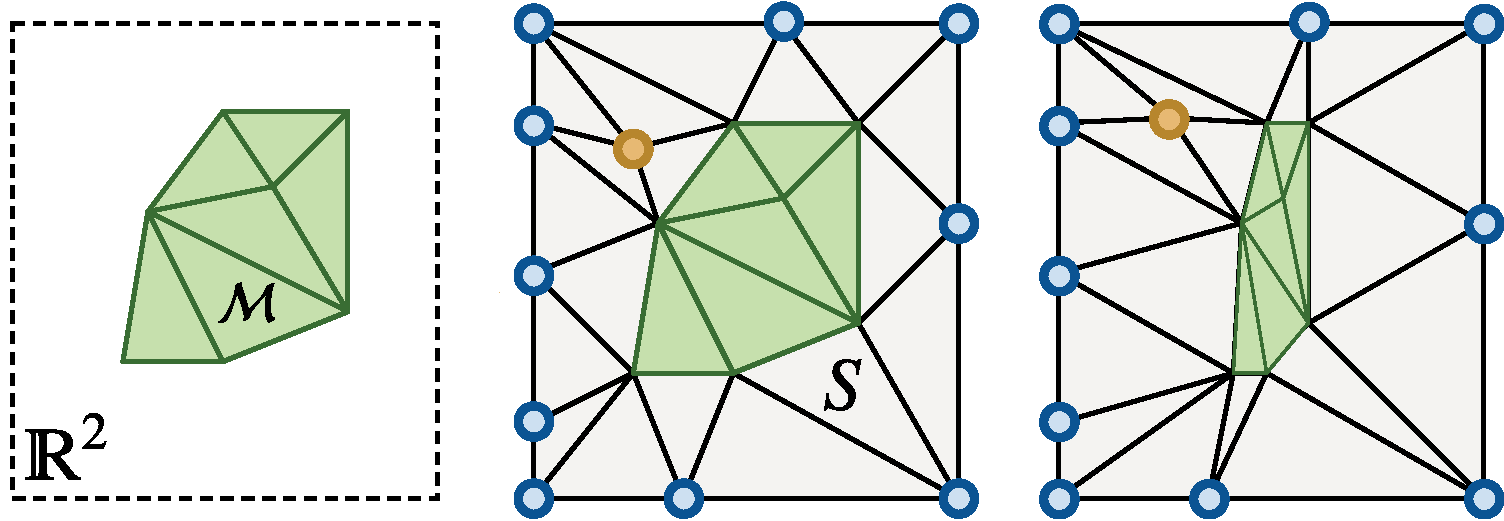
\includegraphics[width = \columnwidth]{scaf-tex/figs/scaffold_illustration}
\caption{The initial mesh $\Mesh$ (in green, left), is embedded in another mesh $D$ (in gray, middle) that covers a box in the ambient space and contains the same triangles as $\Mesh$. $D$ might contain additional points (orange). We denote the triangles that are in $D$ but not in $\Mesh$ as the scaffold $S$. Our algorithm deforms $D$, inducing a corresponding deformation on $\Mesh$ (right), while keeping the boundary (blue vertices) fixed and preventing changes in the triangle orientation.}
\label{scaf:fig:construction}
\end{figure}


 \paragraph{Variational Formulation} 
 Minimizing the distortion of $\Phi$ using the augmented map $\Psi$ poses an interesting challenge: what is the desired shape of the scaffold $S$? Ideally we would like the simplices in the scaffold to maintain their orientation and not affect the optimization in any other way. Such a requirement is difficult to model directly, since it is a discontinuous condition that is not well-suited for the variational framework that we would like to use to minimize $E_{\Mesh}$. 
 
 We propose a regularized version of this condition modeled with an energy $E_{\Mesh} (\Psi|_{S})$ that still diverges when elements change orientation and that mildly penalizes any non-rigid distortion.
 
 We choose a reweighted version of the symmetric Dirichlet energy $\Distort$~\cite{Smith:2015}, measured w.r.t. the Jacobian of the map $\Psi$ computed from the rest pose of $S$ for each simplex $f$,
\begin{equation}
    J_f := \nabla \Psi_f
\end{equation}
where $\Psi_f$ is the restriction of $\Psi$ over the simplex $f$, which is an affine map. We divide the energy of each scaffold simplex $f$ by its area $A_f$, and sum them up to obtain the final energy that favors an equal contribution regardless of the size of each scaffold simplex:
\begin{align}
    \begin{split}
    E_S(\Psi|_{S}) =&\sum_{f\in S} \frac{1}{A_f} \Distort(J_f) \\
    =&\sum_{f\in S} (\norm{J_f}_F^2 + \norm{J^{-1}_f}_F^2 -2d).
    \end{split}
\end{align}
The $-2d$ term ensures that the energy is 0 when $J_f = \mathbb{I}$. The map is then computed by summing the two terms:
\begin{align}
\begin{split}\label{eq:variational}
\min_{D} & \quad E_{\Mesh}(\Psi|_{\Mesh}) + \lambda E_{S} (\Psi|_{S}) \\
    \text{s.t.} & \quad \Psi|_{\partial D} \revision{\text{ is Identity}} \\ 
    & \quad \Psi \text{ preserves orientation}.
\end{split}
\end{align}
where $\lambda > 0$ is balancing the contribution of the two energies, decreasing as the optimization proceeds.

\paragraph{Iterative Regularization}
Solving this problem leads to a bijective and distortion minimizing map, but the regularizer will affect the stationary points of $E_{\Mesh}$, which is problematic, especially for large deformations.
%
To address this problem we iteratively minimize this energy, regenerating the scaffold at each iteration, and use the new scaffold as a rest pose for the regularization term $E_{S} (\Psi|_{S})$. This iterative procedure has two positive effects: (1) it acts as a proximal regularization term without inhibiting movement since the rest pose is updated at each iteration; (2) the meshing quality of the scaffold is high, which avoids locking configurations.

\paragraph{Interpolation Coefficient.}
We experimentally observed that our algorithm is robust to different choices of $\lambda$, generating indistinguishable results in most cases. However, $\lambda$ affects the convergence speed (Figure \ref{scaf:fig:different_weight}). We used $\lambda = \frac{1}{100}\frac{ E_{\Mesh}(\Psi|_{\Mesh})}{|S|}$ for all our experiments, where $|S|$ is the number of scaffold simplices.

\begin{figure}[h!]
\centering
    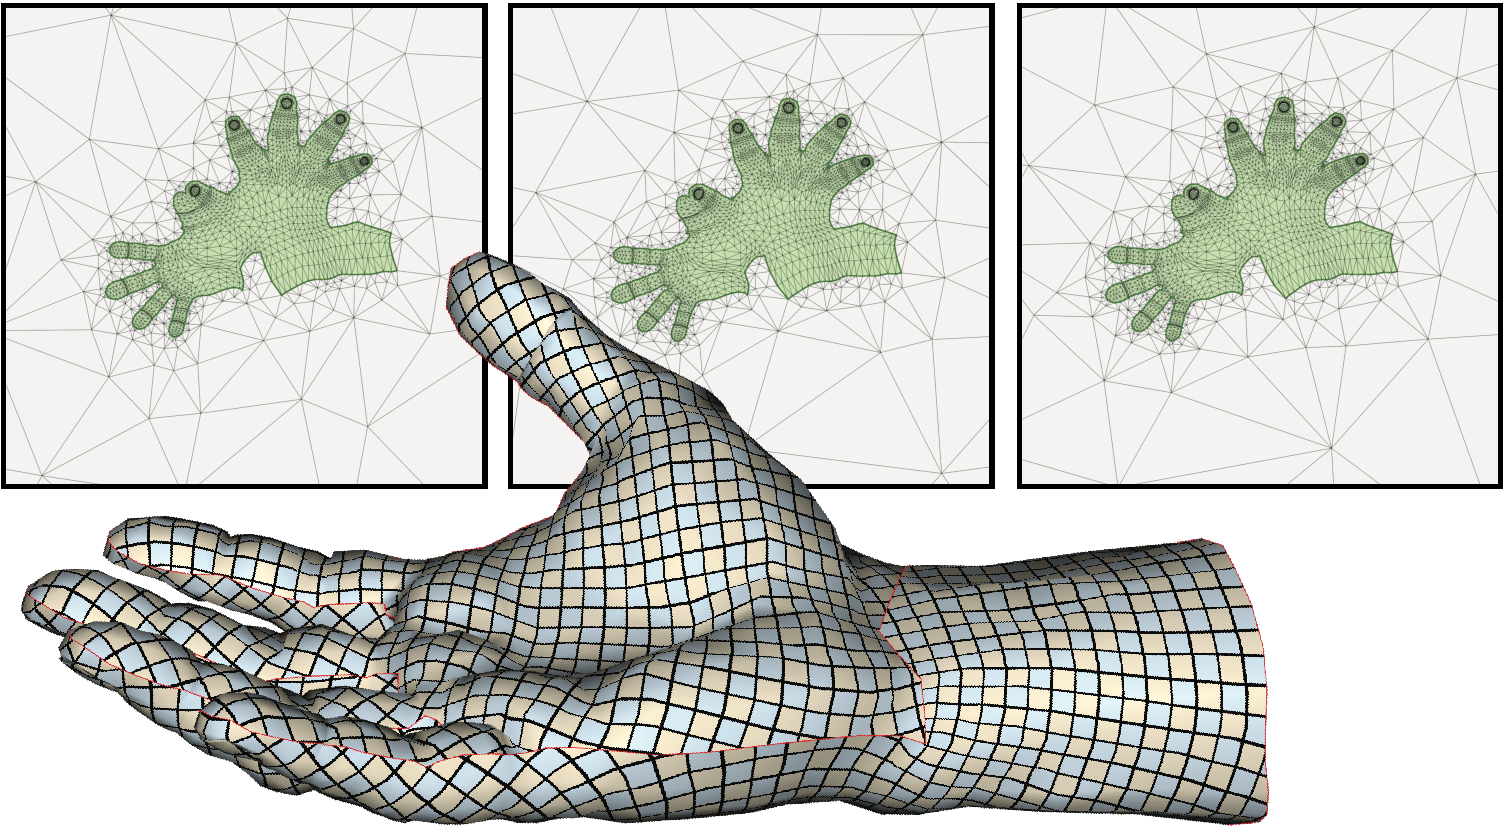
\includegraphics[width = \columnwidth]{scaf-tex/figs/hand_weight}
\caption{Different values of $\lambda$ do not affect the result, but they change the number of iterations needed. From left to right: we used a large weight (100x ours), our weight, and a small weight (0.01x ours). The optimization took 9,7, and 8 iterations, respectively, to reach the same energy level.}
\label{scaf:fig:different_weight}
\end{figure}

\paragraph{Solver.}
Since our energy is rotational invariant, we can minimize the energy with the same quadratic proxy proposed in SLIM \cite{Rabinovich:2017}, enriching the approach with the equality constraint needed to fix the boundary $\partial D$. We also employ the orientation-preserving line search \cite{Smith:2015} (with exact predicates \cite{Shewchuk:1996}) to ensure that no triangles can change orientation. Alternatively, other methods such as AQP \cite{Kovalsky:2016} could be used to minimize this energy. Since our approach changes the mesh connectivity at every iteration, AQP loses much of its advantages as the approximate \revision{H}essian must be recomputed at each iteration and not prefactored.  Therefore, our approach is an ideal fit for \cite{Rabinovich:2017}, which takes large steps at every iteration without relying on a constant, prefactored matrix at each iteration. For practical applications, SLIM iterations are sufficient to minimize the energy to acceptable levels. For two  stress tests (figures \ref{scaf:fig:recovering} and \ref{scaf:fig:smith}) we used the result of SLIM as a warm start for a Newton optimization (as suggested by \cite{Rabinovich:2017}), which quickly converges to a numerical minimum.

\subsection{Surface Parametrization}
Our framework can be used for many applications, one of which is computing a bijective surface parametrization from a 3D surface into the UV  plane. We follow \cite{Liu:2008} and assume that each 3D triangle $f^{3D}$ is equipped with a rigid transformation $R_f$ such that applying $R_f$ to $f^{3D}$ maps $f^{3D}$ to the plane. Given this transformed triangle $f$, we can now measure the distortion of the map using the Jacobian of the affine transformation (a $2\times2$ matrix) from $R_f(f^{3D})$ to $f$, the location of the triangle in the parametrization.

\paragraph{Initialization} Our method is initialized with Tutte's embedding algorithm~\cite{Tutte:1963}:
\[\Phi^0 : \Mesh^{3D} \rightarrow \Omega^0,\]
where $\Omega^0$ is a simplicial disk domain. Then we construct a larger rectangular domain $D^0 \supset \Omega^0$, where $\partial D^0$ is an axis-aligned rectangle, and use Triangle \cite{Shewchuk:1996} to triangulate the region in between.  We enforce a quality bound of $20^\circ$ to obtain a graded mesh that is coarse on the boundary and conforming the boundary of $\Omega^0$. This grading implicitly produces an approximate inverse distance  weighting of the scaffold space with respect to the error function, which enables a larger deformation per iteration. Then we define $\Psi: D^0 \rightarrow D \subset \mathbb{R}^{2}$ and restrict $\Psi |_{\partial D^0}$ to be the identity.
% \DP{Can we drop this?}We denote the vertex coordinates in $D^0$ by $U^0$, and augmented face set by $\matS$, i.e., $D^0 = (\matU^0, \matF\cup \matS)$.

\paragraph{Mesh Improvement}
At the end of each iteration, we improve the quality of the scaffold. The reason for maintaining a good mesh quality is two-fold. 
First, as observed in \cite{Zhang:2005, Muller:2015}, fixing the scaffold will potentially prevent movement. Secondly, the quality of the scaffold affects the condition of the linear system in SLIM \cite{Rabinovich:2017}: a higher  quality leads to larger and more efficient iterations.

We resort to Triangle \cite{Shewchuk:1996} to create the initial scaffold and to regenerate the scaffold mesh in the improvement step. Our experiments show that, in 2D, it is faster to generate the mesh from scratch at every iteration instead of trying to optimize the scaffold using local operations as suggested in \cite{Muller:2015}. Since our solver makes large steps in each iteration, the scaffold requires significant connectivity changes each iteration, which explains why regenerating the triangulation is faster than local operations. This is in stark contrast with physical simulation scenarios where each iteration represents a small time step and, thus, a minor change in the vertex positions.

We demonstrate the effectiveness of the remeshing strategy in Figure \ref{scaf:fig:recovering} where our method recovers from a large rotation --- note that the scaffold is updated during the iterations and always leaves space for the map to move freely.

\begin{figure}[h]
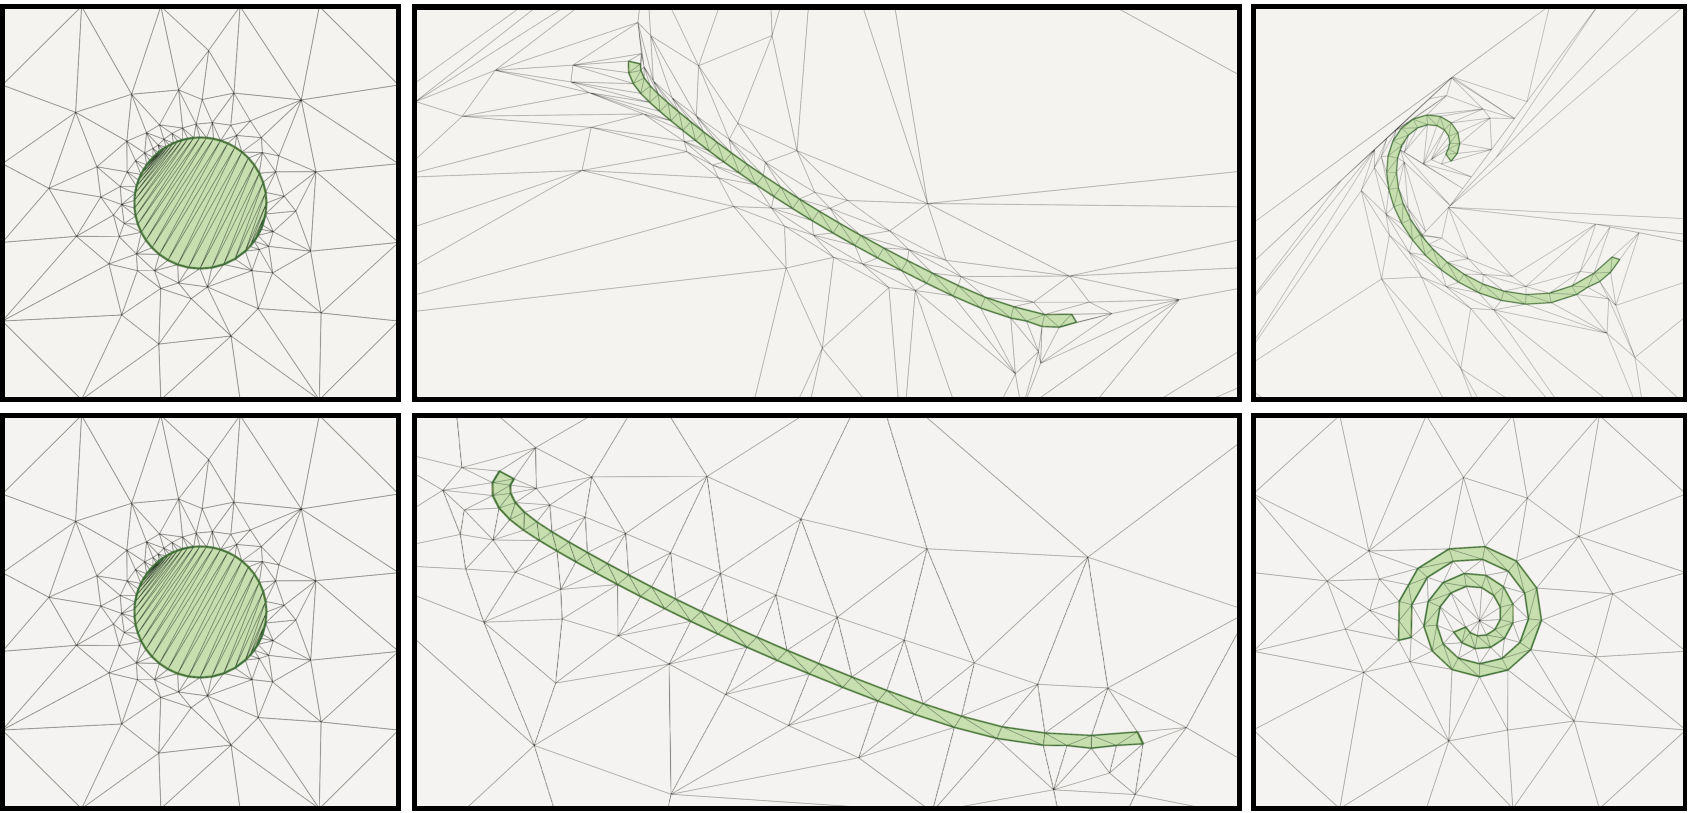
\includegraphics[width=\columnwidth]{scaf-tex/figs/coil-remeshing}
\caption{
\label{scaf:fig:recovering}
A bijective map from a circle (left) to a spiral (right) is computed without (top) and with (bottom) the iterative remeshing step. The slivers in the triangulation locks the optimization (top), preventing it from reaching the target shape.
% Recovering from a large rotation (up is remeshing: init, 30SLIM, 30 Newton; down is w/o reeshing 30 SLIM, 270 Newton) 
}
\end{figure}
\paragraph{Sliding \revision{\& Degeneracy Prevention}}
As the optimization proceeds and some of the boundary elements get closer, some of the scaffold triangles might (and often will) get smaller and smaller, restricting the amount of sliding that is allowed in one iteration as well as introducing numerical difficulties in computing the corresponding Jacobian $J_f$ \revision{whose singular values will approach infinity.}
% (Figure \ref{scaf:fig:slide}).  

To avoid this issue, we replace the degenerating target \revision{when computing its} Jacobian. For the triangles with an area smaller th\revision{an $\epsilon$, we use an equilateral triangle with area $\epsilon$ to compute the local Jacobian.} \revision{In our experiment,} we traverse through the boundary of the interior of the uv domain at the current iteration to find the minimum edge length $l$ \revision{and set} $\epsilon = \frac{l^2}{4}$.

A theoretical downside of this modification \revision{is that} it affects the distortion energy. We experimentally observed that the changes are negligible, and we thus used it for all our experiments. \revision{However, on the practical side}, it discourages fully degenerate elements --- this change, coupled with the orientation preserving line search \cite{Smith:2015}, makes our algorithm robust \revision{enough for the challenging stress tests shown in} Figure \ref{scaf:fig:miq_database}.
% \begin{figure}{h}
% 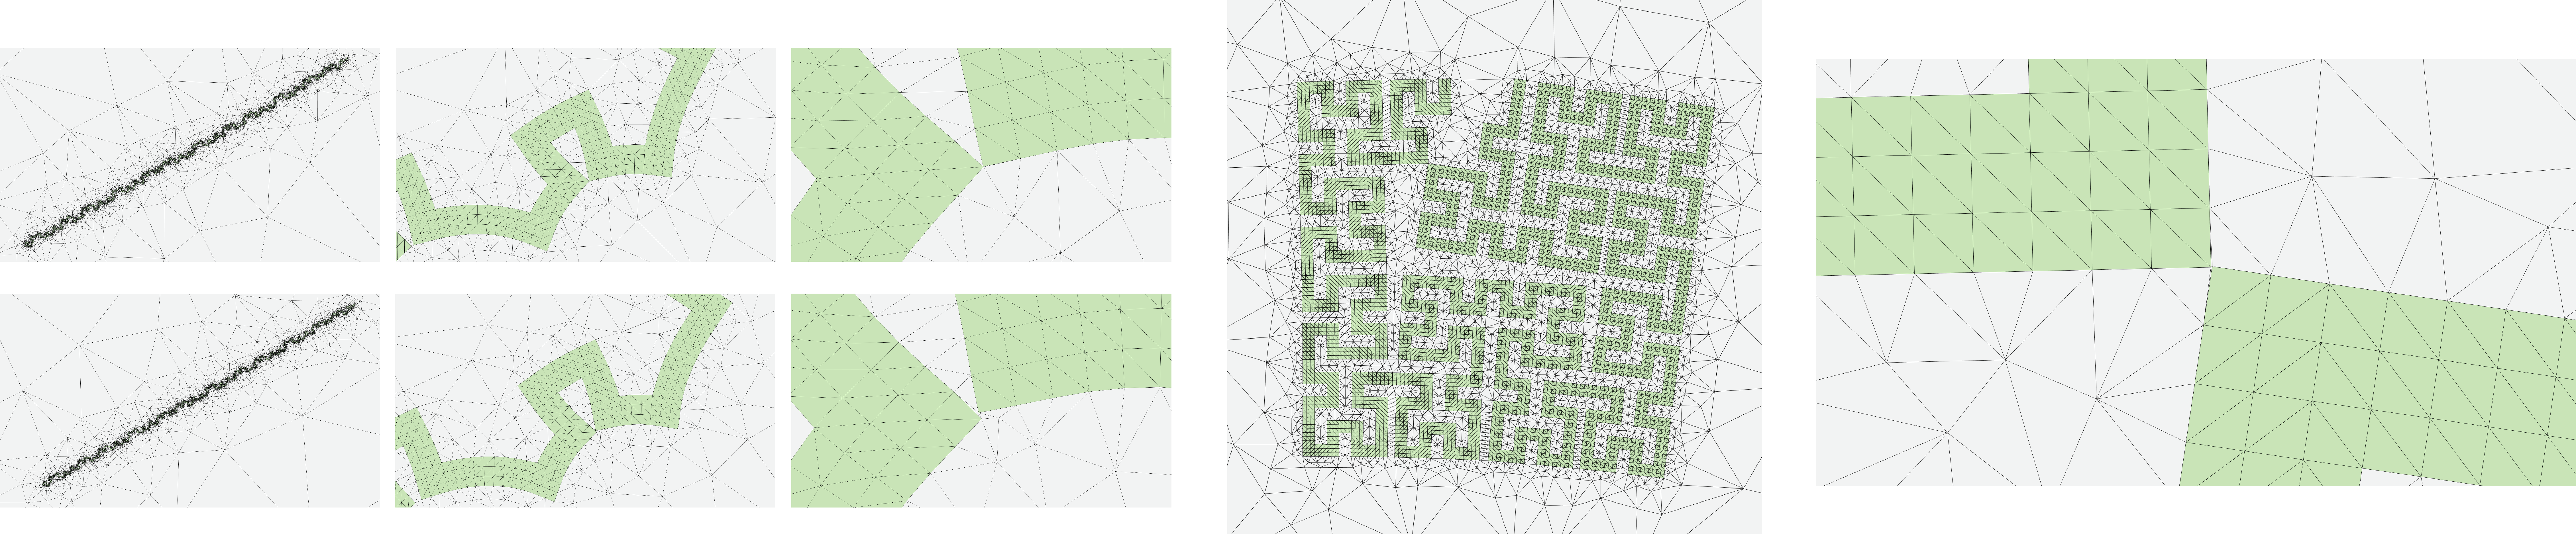
\includegraphics[width=8cm,height=4cm]{scaf-tex/figs/hilbert_area_threshold}
% \caption{
% Sliding example, one gets stuck the other one does not. \DP{TODO}}
% \label{scaf:fig:slide}
% \end{figure}

\subsection{Extension to 3D}

\revision{Our formulation naturally unifies bijective geometric optimization problems in 2D and 3D, so the} algorithm readily extends to the 3D case with only one major difference: the scaffold becomes a tetrahedral mesh, which is computationally more challenging to create and update.
\paragraph{\revision{Mesh Improvement}}
We use TetGen \cite{Si:2015} to generate the initial scaffold and the local operations proposed in \cite{Klingner:2009} to optimize the scaffold's quality in the subsequent iterations. 
%We describe our mesh improvement algorithm in details in Appendix \ref{appendix:improvement} \DP{TODO}.
%
It is unfortunately not possible to directly use TetGen at every iteration as we did with Triangle in the 2D case, since TetGen fails when boundaries get too close, which is common in our experiments.

\revision{
\paragraph{Guarantee} Similarly to the 2D case, we are guaranteed that no flipping or self-intersecting tetrahedra will occur since we are following an interior point strategy. Notice the contrast with Air Mesh \cite{Muller:2015} where only if penetration happens can the constraints be of effect. However, as pointed out in \cite{Dougherty2004}, the local operations we are performing may not be sufficient to explore the entire space of possible tetrahedralizations. %effective enough to explore the whole space of tessellation. 
Therefore, we cannot guarantee that the algorithm achieves the globally optimal solution.
}
%\input{sections/discussion}
\section{Results}
We implemented our algorithm in C++ using Eigen for linear algebra routines. We \revise{ran} our experiments on a desktop with a 4-core Intel i7  processor clocked at 4 GHz and 32 GB of memory \revise{but using only one thread on a single core}. For all experiments, the scaffold bounding box is computed by uniformly scaling by three times the bounding box of the image of the current map. 

\begin{figure}[t]
\includegraphics[width=8cm]{figs/database_demo}
\caption{Two models are cut using \cite{Bommes:2009} and bijectively parametrized using our algorithm. See the additional material for more examples.}
\label{scaf:fig:miq_database}
\vspace{-0.2cm}
\end{figure}

\paragraph{Robustness.} To demonstrate the robustness of our algorithm, we computed  bijective maps for all the 102 meshes parametrized by the MIQ algorithm \cite{Bommes:2009} \revise{and for the 17 meshes parametrized by  \cite{Myles:2014}} in the dataset proposed by \cite{Myles:2014}. The cuts in these meshes have been designed for locally injective parametrization that usually have major self-overlap. We use them as a stress test for the effectiveness and robustness of our method:  the cuts introduce a massive distortion in the Tutte initialization and lead to boundaries that are prone to overlap in hundreds of locations. Our method successfully creates bijective parametrizations for all these models with default parameters. We attach all the parametrized models in the additional material and show two examples in Figure \ref{scaf:fig:miq_database}. 


% To demonstrate robustness in 3D, we deform \DP{XX} surfaces simultaneosly, by prescribing positional constraints that are  We simulate the deformation of a material made of hundreds of elastic layers. We run the simulation both on a 2D slice and on the full 3D model in Figure \ref{scaf:fig:stresstestlayers}. For this example, we compare the result obtained with the SLIM solver proposed in this paper and with the AQP algorithm \cite{}. \DP{TODO after we will know how it looks.}

% \begin{figure}[h]
% 
\includegraphics[width=8cm]{figs/placeholder.png}
% \caption{Mille-feiulle, both in 2D and 3D \DP{TODO}}
% \label{scaf:fig:stresstestlayers}
% \end{figure}

\paragraph{Scalability.} Our methods scales gracefully to large datasets, similarly to \cite{Rabinovich:2017}. We repeat their scalability experiment, but producing bijective maps instead of just locally injective maps (Figure \ref{scaf:fig:scalability}). The behaviour is remarkably similar --- the density of the model (and consequently of the scaffold) does not affect the number of required iterations. 

\begin{figure}[t]
\includegraphics[width=\columnwidth]{figs/lucy-scalability}
\caption{We compare the distortion energy with respect to the number of iterations on a set of Lucy's meshes with different resolutions (from 1 to 12 million faces). In the center of the plot, we show the 1M Lucy model parametrized by our algorithm.
}
\label{scaf:fig:scalability}
\end{figure}

\paragraph{Texture Atlas Generation} 

UV mapping is a time consuming procedure required in most geometric modeling pipelines. Existing commercial tools provide the ability to flatten single patches and arrange them in UV layouts where multiple patches are tightly packed inside a rectangular domain, which is then loaded in the texture memory of a GPU. 

Our algorithm can bijectively parameterize a single patch (Figure \ref{scaf:fig:manuallycut}), avoiding the typical manual UV postprocessing required with traditional tools.  Our algorithm can also be used to create automatic UV charts of models with multiple connected components (or predefined cut edges). We show an example in Figure \ref{scaf:fig:packing2D} where we detected the connected components, bijectively map the patches into a set of circles (using a grid layout), and reduce their distortion using our algorithm. The result is a tight and automatic packing without resorting to any user-interaction. Additional interactive tools can further improve the atlas by dragging\&dropping regions or translating islands while ensuring that no overlaps are introduced (Figure \ref{scaf:fig:teaser}). We show interactive sessions using our packing tool in the additional material.

\begin{figure}[t]
\includegraphics[width=8cm]{figs/the_animal}
\caption{A mesh is cut by an artist into a single chart and parametrized using SLIM \protect\cite{Rabinovich:2017} (left) and with our algorithm (right). Note that local-injectivity is not sufficient for this model, since the global overlaps in the highlighted region prevent this parametrization from being a UV texture map. Our result (right) is guaranteed to be bijective.}
\label{scaf:fig:manuallycut}
\vspace{-0.2cm}
\end{figure}

\begin{figure}[t]
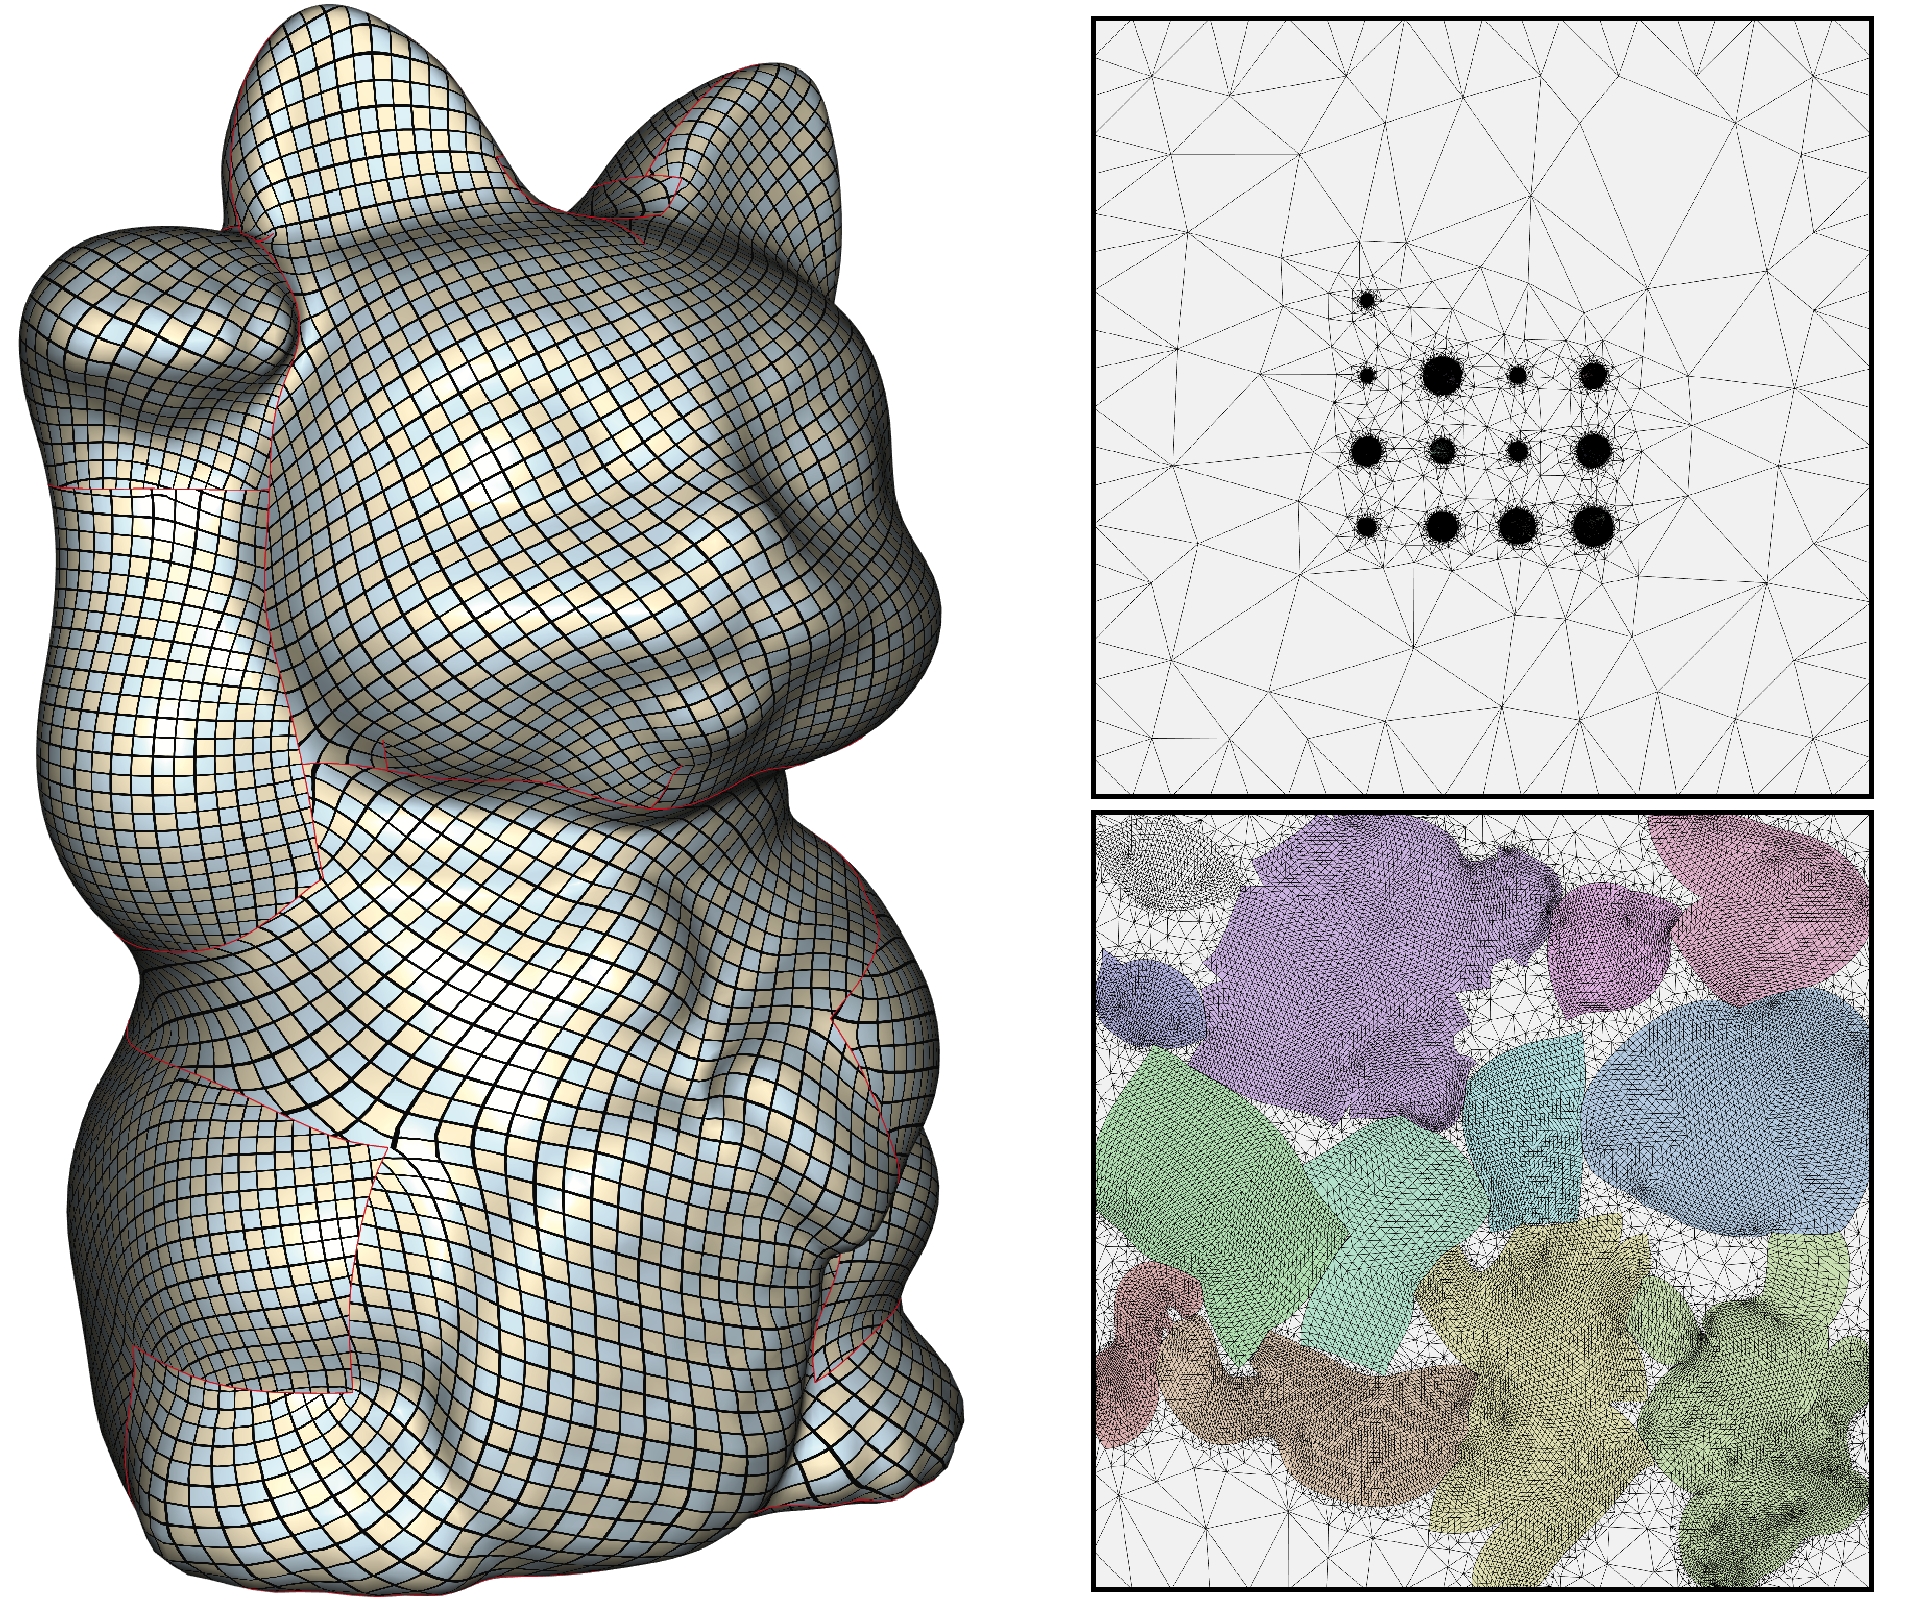
\includegraphics[width=\columnwidth]{figs/maneki_neko_colorful}
\caption{A model with multiple chart (left) is automatically parametrized in a texture atlas (bottom-right) by first mapping each component to a circle (top-right) and then minimizing the distortion.}
\label{scaf:fig:packing2D}
\end{figure}

\paragraph{Preventing Self-Intersections}
Our algorithm can be generalized to handle mixed dimension problems, such as the deformation of 2D surface in 3D space, while preventing self-intersections. In Figure \ref{scaf:fig:flow}, we demonstrate the use of our method to resolve self-intersections of surfaces. First we perform a conformalized flow \cite{Kazhdan:2012} using the algorithm proposed in \cite{Sacht:2013} to resolve any self-intersections.  While \cite{Sacht:2013} will resolve the intersections, the resulting surface may be geometrically far from the initial shape (see Figure \ref{scaf:fig:flow}).  Next we tetrahedralize the ambient space while conforming to the deformed surface mesh and minimize Equation \ref{eq:variational} with an additional energy term that strives to restore the rest pose geometry of the surface, using the surface ARAP energy proposed in \cite{Sorkine:2007}. The result is a surface similar to the original mesh, but without self-intersections. In this example, it is possible to observe that even dramatic changes of scale (on the foot) can be robustly handled by our parametrization algorithm.

A more challenging stress test is shown in Figure \ref{scaf:fig:rabbit}, where the bunny model is scaled up inside a box, to 30 times its original size. No self-intersections are introduced, despite the extreme, constrained deformation.

\begin{figure}[t]
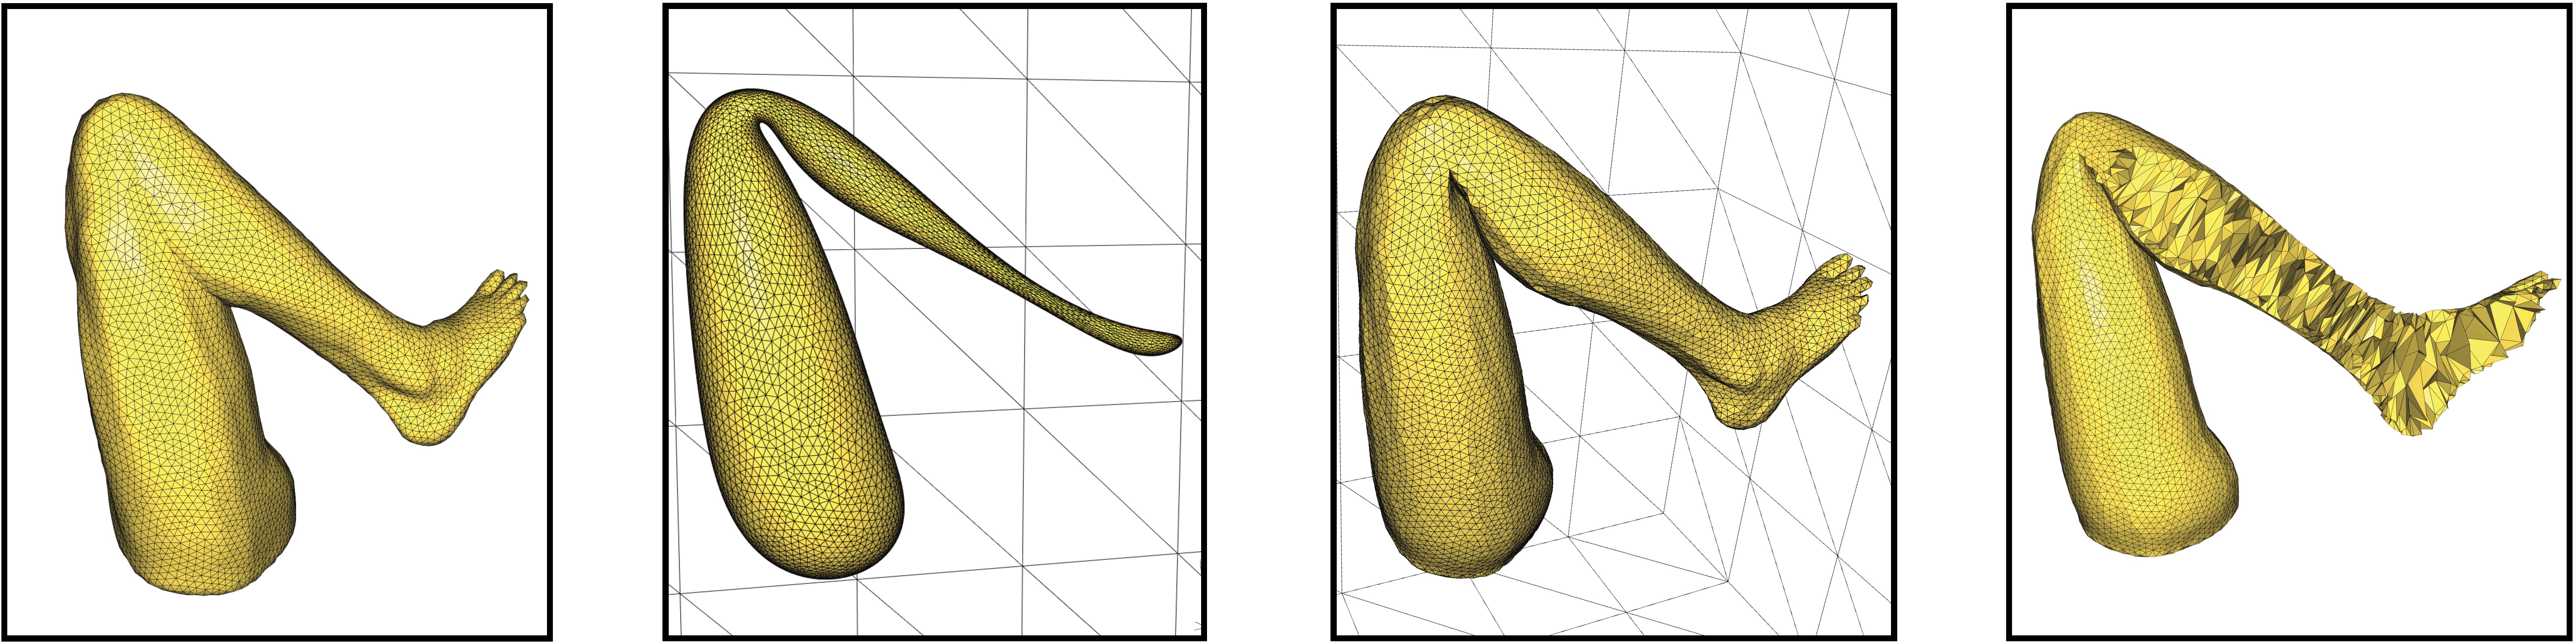
\includegraphics[width=\columnwidth]{figs/leg-flow}
\caption{We remove the self-intersections from a genus 0 model using the conformalized flow \protect\cite{Kazhdan:2012,Sacht:2013}. The flow is inverted, while using our algorithm to compute a bijective volumetric map, to recover a self-intersection free version of the original surface. The final model can now be meshed using TetGen, since it is free from self-intersections.}
\vspace{-0.2cm}
\label{scaf:fig:flow}
\end{figure}

\begin{figure}[t]
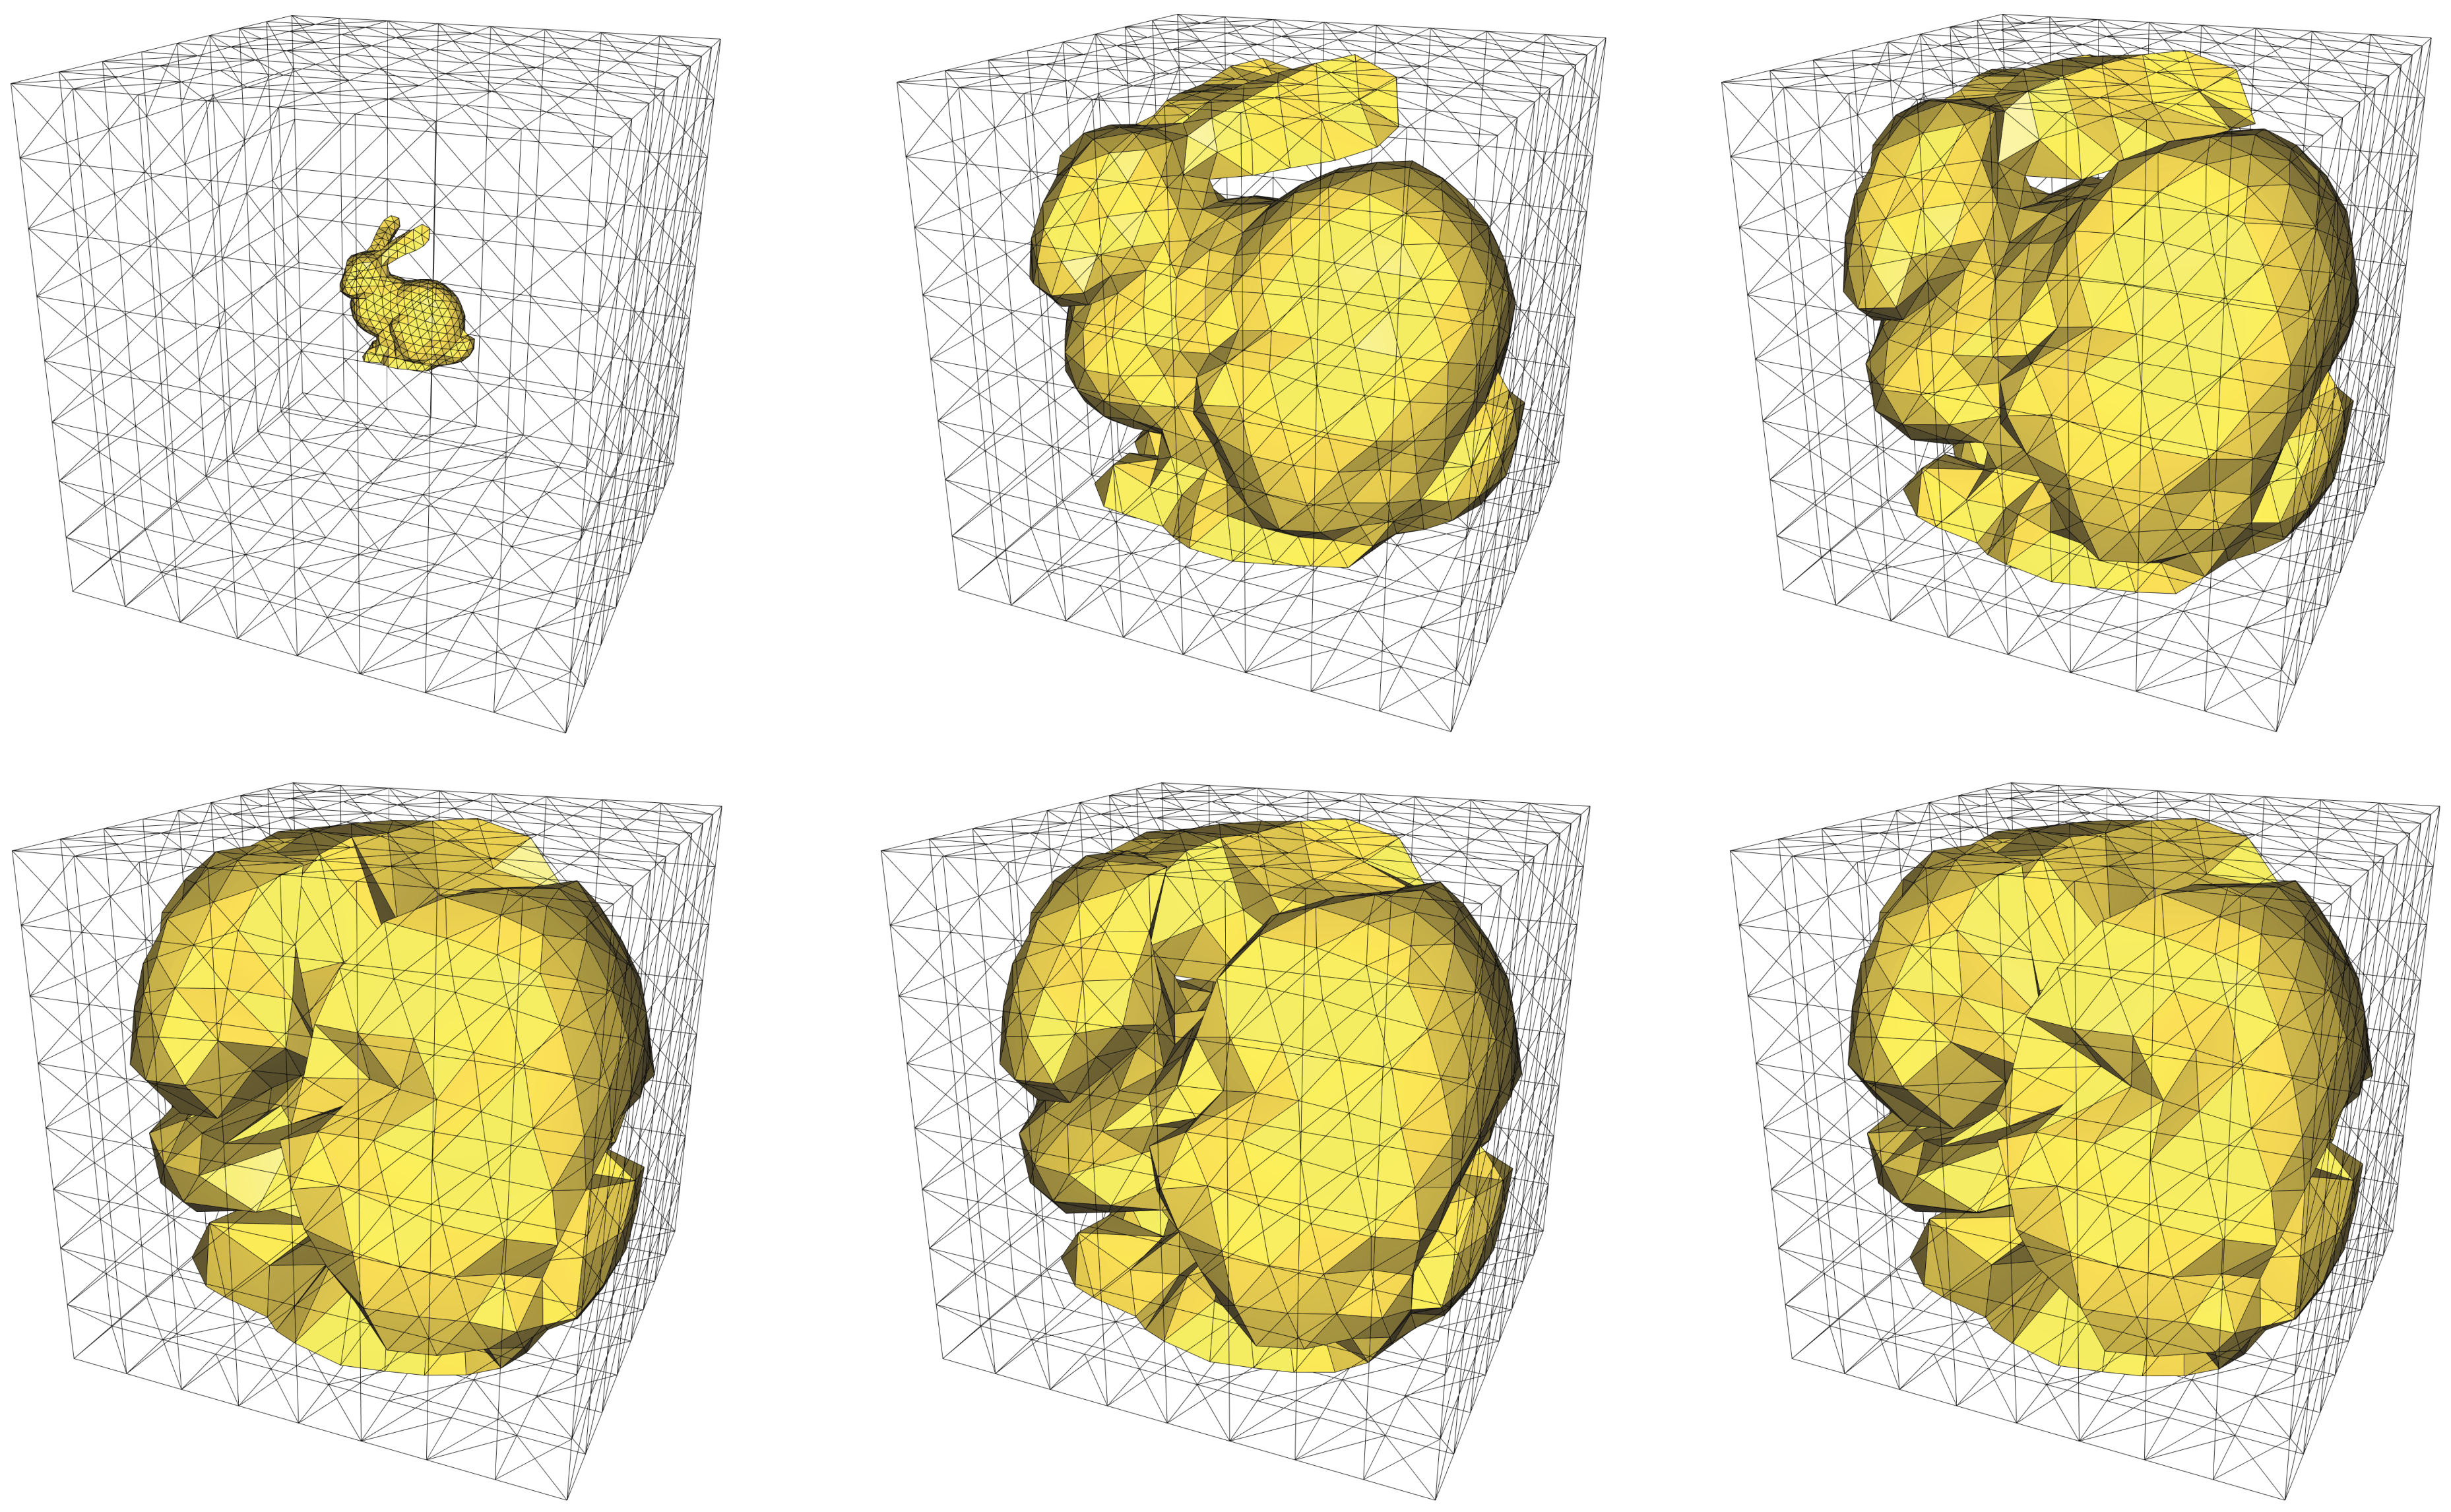
\includegraphics[width=0.8\columnwidth]{figs/rabbit_grow}
\caption{We grow a bunny inside a box, while preventing  self-intersections. We show the result after 0,10,20,30,40, and 50 iterations.}
\label{scaf:fig:rabbit}
\end{figure}


\paragraph{Comparison with \cite{Smith:2015}}
The algorithm closest to ours is \cite{Smith:2015}, which tackles a similar problem (restricted to the 2D case). We replicated the space filling curve experiment and obtained remarkably similar results, where our running time is 96s, compared with 8,472s for \cite{Smith:2015} (88 times faster). We show in Figure \ref{scaf:fig:smith} a more challenging experiment with a subdivided version of the space filling curve to emphasize the performance difference: our algorithm converges in 39 minutes, while \cite{Smith:2015} did not converge after 5 days and 21 hours. For this example, we used the procedure suggested in \cite{Rabinovich:2017}: we performed a few iterations minimizing the quadratic proxy and then switch to a traditional newton method until numerical convergence. A video of the optimization is provided in the additional material.

\begin{figure}[t]
\includegraphics[width=\columnwidth]{figs/dense_hilbert}
\caption{\revise{We repeat the challenging test in \cite{Smith:2015} with a subdivided version of their Hilbert curve to increase the triangle count. Our method starts from a disc (upper left), gracefully extends (upper right), and reaches the same minimum (lower left) in 39 minutes whereas \cite{Smith:2015} didn't terminate more than 5 days (lower right), highlighting our performance boost of over 200 times.
}}
\label{scaf:fig:smith}
\vspace{-0.2cm}
\end{figure}

\begin{figure}[t]
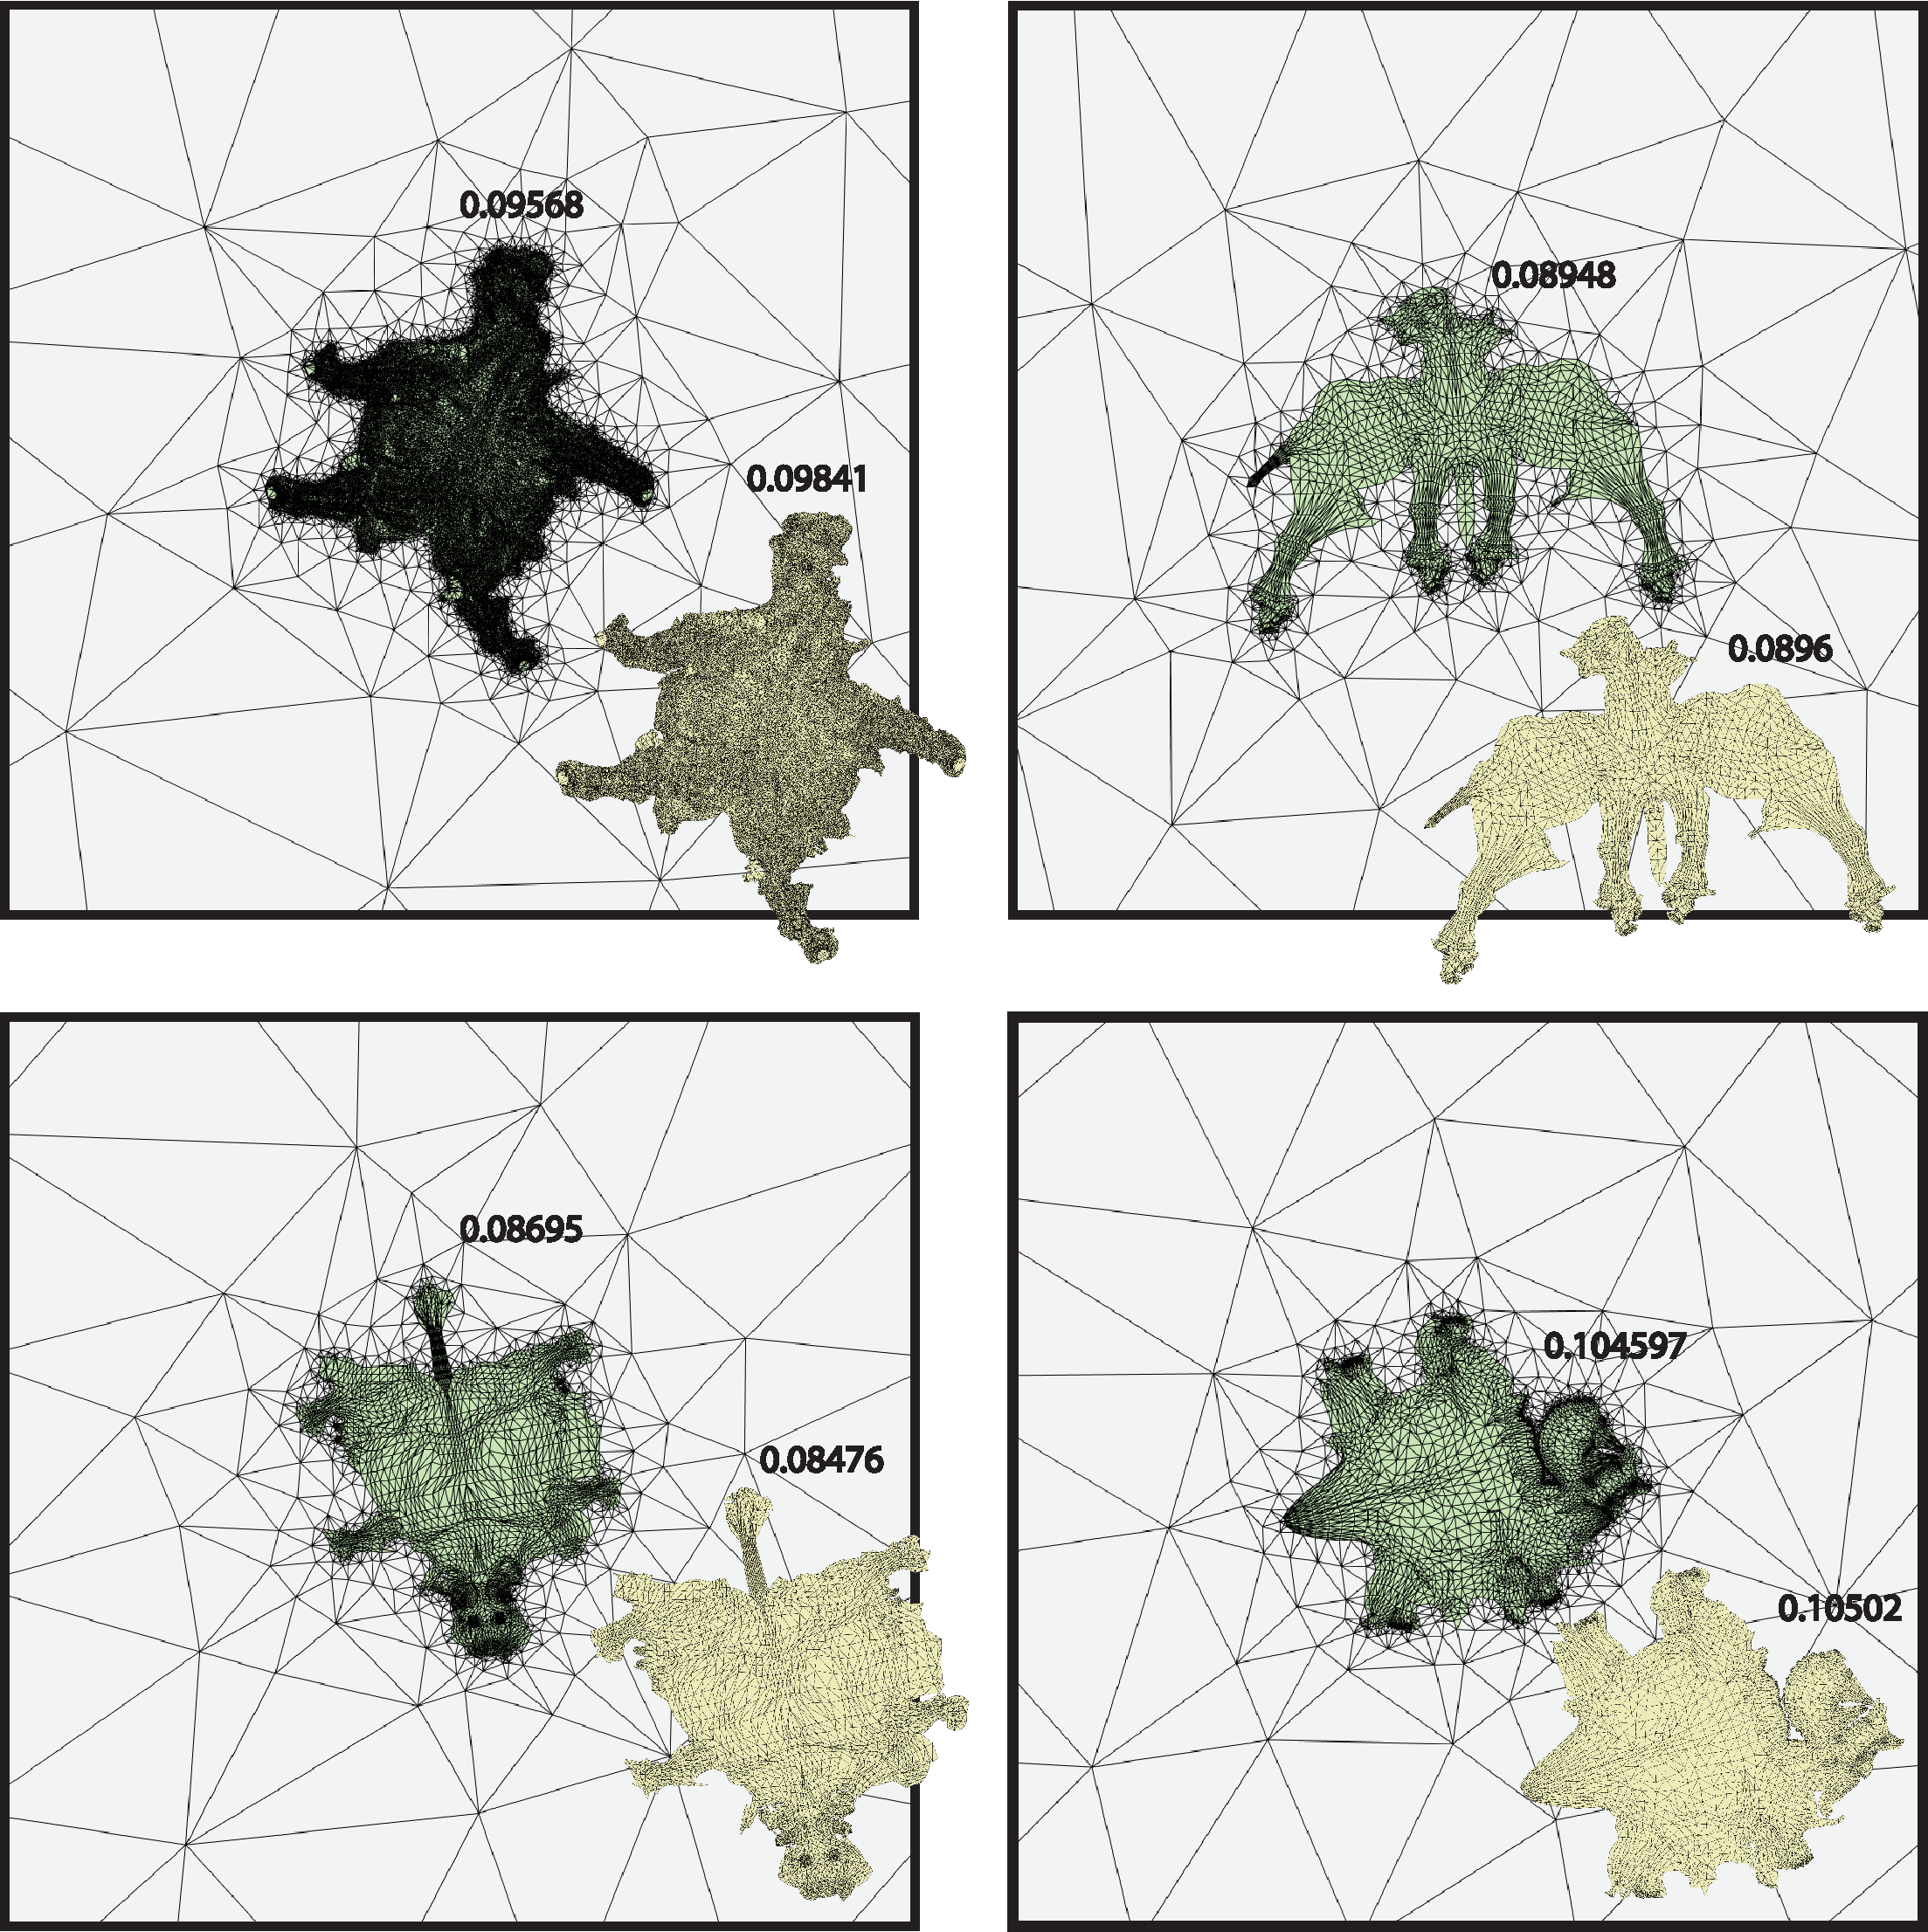
\includegraphics[width=\columnwidth]{figs/compare_smith}
\caption{\revise{We apply our algorithm on 4 models used in \cite{Smith:2015} (using the same stopping criteria) obtaining visually identical results. Distortion errors produced by our algorithm (outer) and theirs (inner) are shown in black.
}}
\label{scaf:fig:smith-all}
\vspace{-0.2cm}
\end{figure}

\revise{Our method produces results that are visually identical to \cite{Smith:2015}. In Figure  \ref{scaf:fig:smith-all} we repeat the experiments shown in \cite{Smith:2015}, stopping our optimization at the same energy value.}

\paragraph{Local vs Global Optimization} 

Both \cite{Zhang:2005} and \cite{Misztal:2012} use a construction similar to ours to generate bijective maps (Section \ref{sec:related}). Both methods explicitly prevent changes of orientation using a local approach: they optimize the map using coordinate descent iterations \cite{SolomonBook} allowing only one vertex at a time to move in its 1-ring and thus ensuring that no triangle flip. This strategy severely limits the maximal displacement per iteration and restricts the step to the size of the 1-rings. Such a restriction makes these methods impractical for parametrization applications since the difference in scale between the Tutte's embedding and the final result is extreme (the ratio of min and max triangle area is $10^{-6}$ in Figure \ref{scaf:fig:largestep}). We show an example of one of our iterations in Figure \ref{scaf:fig:largestep}, where the highlighted vertex traversed a distance of ~150 times the size of the average edge length of its 1-ring in one single step. Using coordinate descent would have required hundreds of iterations to achieve the same effect. 

\begin{figure}[t]
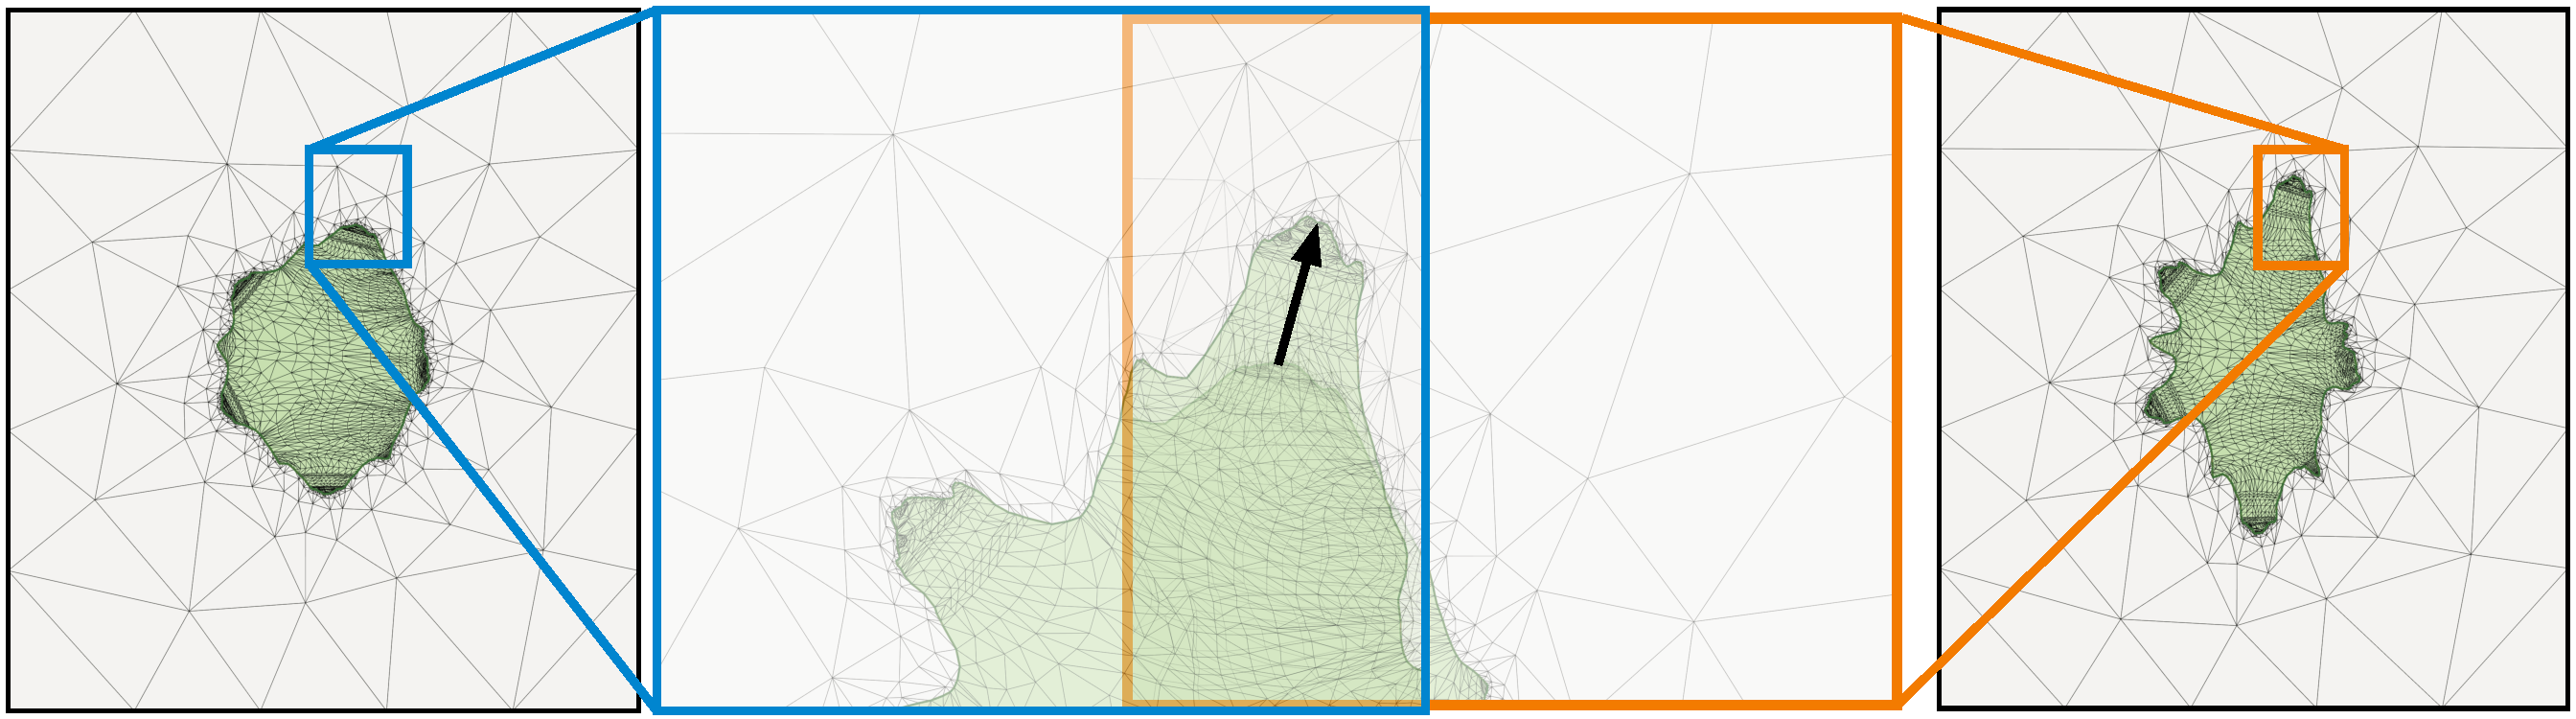
\includegraphics[width=\columnwidth]{figs/camel_step.pdf}
\caption{A single iteration of our algorithm (from left to right) drastically reduces the distortion. The black vector in the center is ~150 times longer than the average edge length of its 1-ring. Iterative methods would need thousands of iterations to achieve a similar progress.}
\vspace{-0.3cm}
\label{scaf:fig:largestep}
\end{figure}

\revise{
% what about... the original is convoluting the metric on the scaffold with the independence to orientation
Despite the orientation-dependent box used as scaffold boundary, our optimization produces results that are, in practice, independent of orientation.  We show this effect in Figure~\ref{scaf:fig:random-rotate} where we initialize the optimization with 1000 randomly rotated Tutte's mappings of the same camel model and run our optimization.  The isometric distortion of the model after 50 iterations is quite similar in all trials (the minimum, maximum, average, standard deviation of distortion errors in all 1000 runs are 0.1086, 0.1107, 0.1095, 3.2698e-4 resp.) indicating very little change based on the initial orientation.
%Since we enforce an isometric energy to the scaffold, translation and rotation is encouraged to make space for the evolving interior boundary. We are able to observe this effect by performing the experiment in Fig. \ref{scaf:fig:random-rotate}. Our algorithm is initialized with 1000 randomly rotated Tutte's mappings of the same camel model, then the isometric distortion of the model after 50 iterations is similar enough (the minimum, maximum, average, standard deviation of distortion errors in all 1000 runs are 0.1086, 0.1107, 0.1095, 3.2698e-4 resp.), indicating very little change based on the initial orientation.
}
\begin{figure}[t]
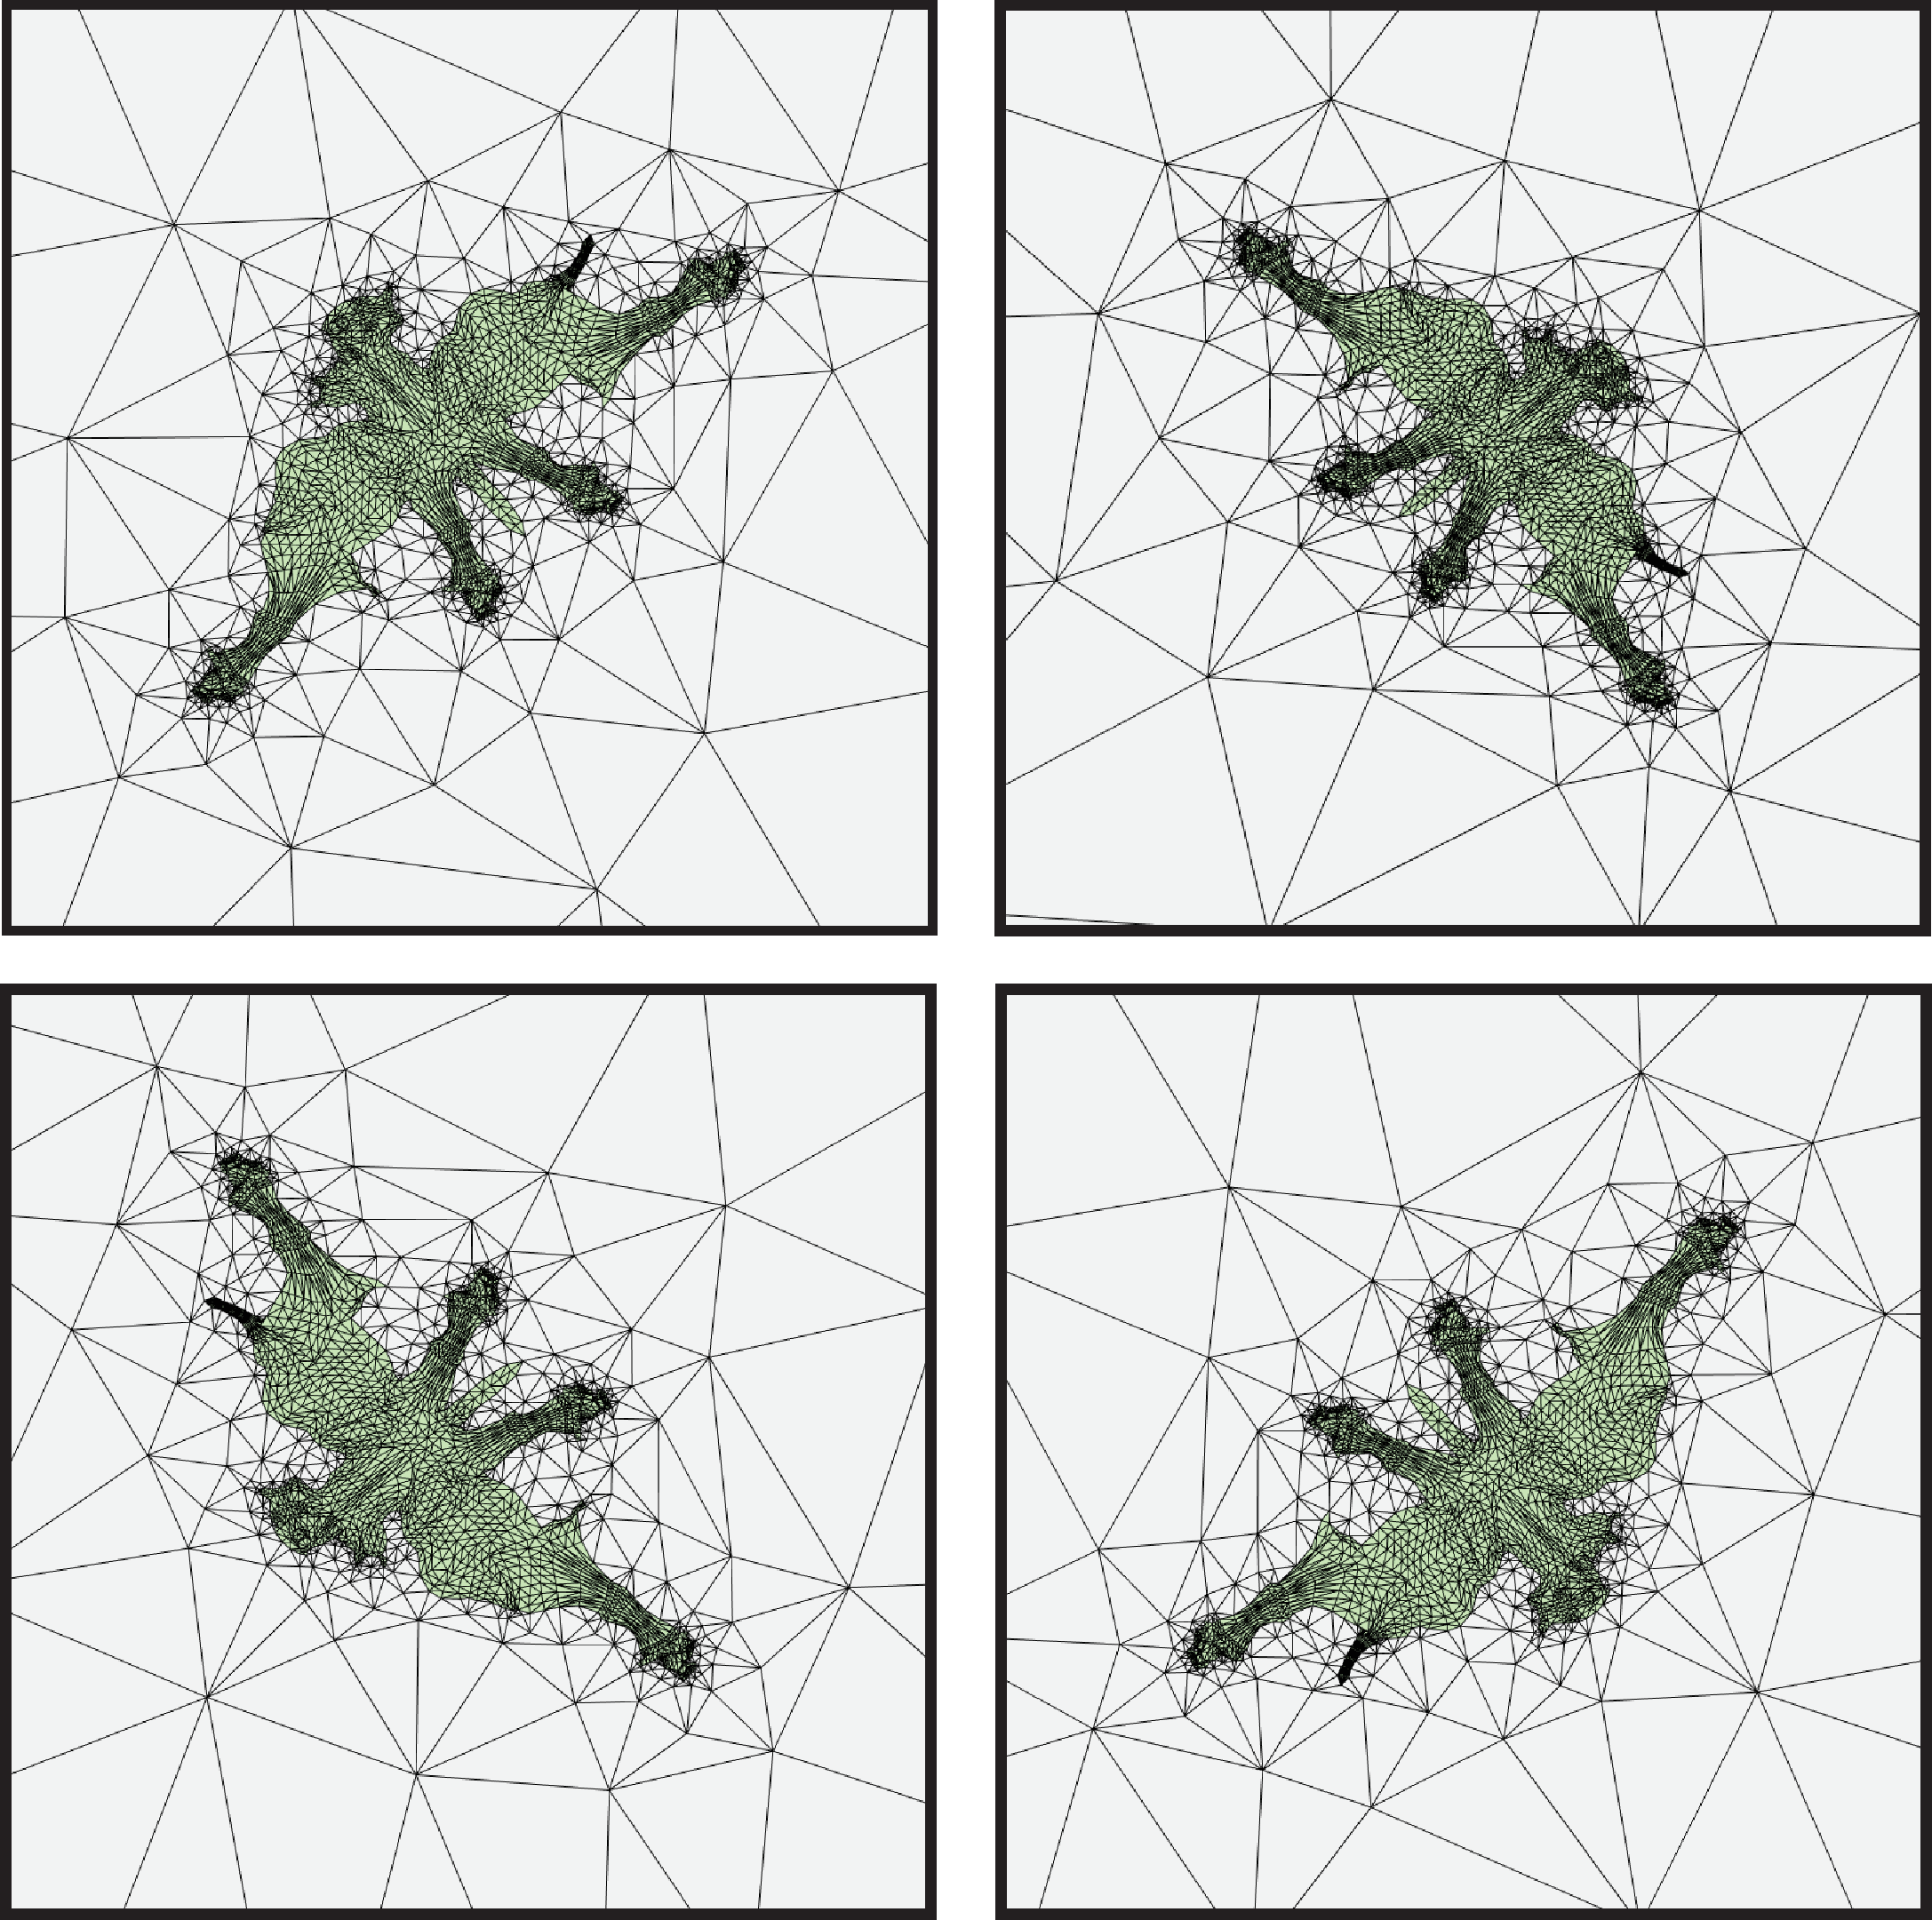
\includegraphics[width=\columnwidth]{figs/random-rotate.pdf}
\caption{
\revise{Our algorithm is independent to the initial orientation. We rotate the initializing Tutte's mapping of the camel model and obtain results with similar isometric distortion.}}
\vspace{-0.2cm}
\label{scaf:fig:random-rotate}
\end{figure}


\paragraph{Timings} The timings for all the results in the paper are reported in Table \ref{tab:timings}.
\begin{table}[t]
	\centering
	\begin{adjustbox}{width=\columnwidth,totalheight=\textheight,keepaspectratio}
	\begin{tabular}{llrrrrrrr}
%		\hline
\textbf{{Type}} &\textbf{Model} & $\mathbf{\#V}$	& $\mathbf{\#F}$ & $\mathbf{\#V_S}$	& $\mathbf{\#F_S}$ & \textbf{It.} & \textbf{{Total Time (s)}} & \textbf{{It. Time (s)}}\\
\hline
\multirow{2}{*}{Atlas}&Nefertiti (Fig.~\ref{scaf:fig:teaser})
&1697	&2823	&983/	247&	1945	/728&	50&	0.71&0.01\\
&Maneki-Neko (Fig.~\ref{scaf:fig:packing2D})
&23025	&43648	&2427	/725&	7174/	3770&	50&	16.81&0.34\\
\hline
\multirow{12}{*}{2D}
&Hand (Fig.~\ref{scaf:fig:different_weight})
&2239&4046&347/280&1104/970&7&0.14&0.02\\
&Spiral (Fig.~\ref{scaf:fig:recovering})
&54&52&78/36&190/106&50(50)&0.04(0.21)&0.01\\
&Thai Statue (Fig.~\ref{scaf:fig:miq_database}, left)
&42405&79970    &   3665/1593&12148/8004&50&28.28&0.56\\
&Filigree (Fig.~\ref{scaf:fig:miq_database}, right)
&56062&100000&9160/2627&30422/17356&100&75.99&0.76\\
&Lucy (Fig.~\ref{scaf:fig:scalability})&	501105&	1000000&	1856/	3470&	5900/	5674&	100&	2524.22&25.24\\
&Lucy (Fig.~\ref{scaf:fig:scalability})&	1001375&	1999999&	2284/	4400&	7297/	7133&	100&	7251.00&72.51\\
&Lucy (Fig.~\ref{scaf:fig:scalability})&	2002031&	3999999&	3587/	6930&	11215/	10985&	100&	22500.07&225.00\\
&Lucy (Fig.~\ref{scaf:fig:scalability})&	3002899&	5999999&	5135/	9859&	16047/	15601&	100&	52235.31&522.35\\
&Lucy (Fig.~\ref{scaf:fig:scalability})&	4002816&	8000000&	5140/	10288&	15890/	15918&	100&	59413.14&594.13\\
&Lucy (Fig.~\ref{scaf:fig:scalability})&	5003408&	10000000&	6194/	12231&	19182/	19040&	100&	95247.59&952.47\\
&Lucy (Fig.~\ref{scaf:fig:scalability})&6004111&12000000 & 7357/6418 & 2291/21036 &50 & 78726.05 &1574.52\\
&Animal (Fig.~\ref{scaf:fig:manuallycut})
&19937&39040&747/593&2306/1998&50&15.36&0.31\\
&Space Filling (Fig.~\ref{scaf:fig:smith})
&79545&146832&90815/88237&181608/176452&200(250)&547.13(1836.58)&5.30\\
&Horse (Fig.~\ref{scaf:fig:smith-all}) & 20636 & 39698 & 1343/984 & 4238/3520 & 30(10) & 8.26(12.03) & 0.28(1.20) \\
&Camel (Fig.~\ref{scaf:fig:smith-all}) & 2032 & 3576 & 384/272 & 1234/1010 & 30(10) & 0.52(1.13) & 0.02(0.11) \\
&Cow (Fig.~\ref{scaf:fig:smith-all}) & 3195 & 5804 & 491/277 & 1546/1118 & 30(10) & 0.81(1.74) & 0.03(0.17) \\
&Tricera (Fig.~\ref{scaf:fig:smith-all}) & 3163 & 5660 & 544/329 & 1732/1302 & 30(10) & 0.83(1.77) & 0.03(0.18) \\
\hline

\multirow{2}{*}{3D}&Leg (Fig.~\ref{scaf:fig:flow})
&6617&13230&5016/5021&68521/68544&500&3251.17&6.50\\
&Bunny (Fig.~\ref{scaf:fig:rabbit})
&568&1132&683/706&6209/6289&50&7.16&0.14\\

\hline
	\end{tabular}
	\end{adjustbox}
			\caption{Timings and statistics for the models shown in the paper. From left to right: number of input vertices and simplices, number of initial/final scaffold vertices and simplices, number of iterations, running time in seconds. The numbers in parenthesis refer to the Newton optimization. Note that our timings are considerably higher than those reported in the SLIM paper for the Lucy model since we used the reference implementation in \protect\cite{libigl}, which {does not use} a multi-threaded solver.}
	\label{tab:timings}
	\vspace{-0.2cm}
\end{table}


%\newpage
\section{Limitations and Concluding Remarks}

We proposed a simple and robust algorithm to generate bijective maps, both in 2D and 3D. We demonstrated the practical value of the algorithm in UV mapping and deformation applications, and its robustness with extensive stress tests.

One major venue for future work is the support of hard positional constraints, which are favored over soft constraints in many practical applications. Our current algorithm only supports soft constraints as geometric energy \cite{Schuller:2013}. To support hard constraints we would need to generate a bijective starting point that guarantees those constraints, and then preserve them in our optimization. While bijecive maps with hard constraints can be constructed for a 2D patch homeomorphic to a disk \cite{Weber:2014} and for a 3D volume homeomorphic to a ball \cite{Campen:2016}, the generic solution is still elusive.

In 3D cases, the generation of the initial scaffold is not as robust as in 2D, since TetGen fails for geometries with self-intersections and other imperfections. Our algorithm is also slower in 3D due to larger and denser linear systems, as well as the need for local mesh refinement operations instead of regenerating the entire tetrahedralization. We believe a more optimized and parallel implementation could reduce this overhead, and plan to explore this in the future.
%\vspace{-0.5em}

%slow in 3D\\
%no robust tetrahedralization\\
%no robust initialization\\
%satisfy user-constraints exactly\\
%floating point accuracy locking\\ % we address this with exact predicates, right?
%restricting to rotation-invariant energies\\
%some effect of the scaffold on the map\\  % we kind of already talk about this wrt sliding, mention again?
%minimal separation\\



 \begin{acks}
 The authors would like to thank
 Michael Rabinovich and Roi Poranne for providing the source code and Lucy models for \cite{Rabinovich:2017},
 Leonardo Sacht for providing the source code and Leg model for \cite{Sacht:2013},
 and the anonymous reviewers for their insightful comments and suggestions.
\end{acks}

% Bibliography
\bibliographystyle{ACM-Reference-Format}
\bibliography{scaffold}


\end{document}

